\documentclass[twoside]{book}

% Packages required by doxygen
\usepackage{fixltx2e}
\usepackage{calc}
\usepackage{doxygen}
\usepackage[export]{adjustbox} % also loads graphicx
\usepackage{graphicx}
\usepackage[utf8]{inputenc}
\usepackage{makeidx}
\usepackage{multicol}
\usepackage{multirow}
\PassOptionsToPackage{warn}{textcomp}
\usepackage{textcomp}
\usepackage[nointegrals]{wasysym}
\usepackage[table]{xcolor}

% Font selection
\usepackage[T1]{fontenc}
\usepackage[scaled=.90]{helvet}
\usepackage{courier}
\usepackage{amssymb}
\usepackage{sectsty}
\renewcommand{\familydefault}{\sfdefault}
\allsectionsfont{%
  \fontseries{bc}\selectfont%
  \color{darkgray}%
}
\renewcommand{\DoxyLabelFont}{%
  \fontseries{bc}\selectfont%
  \color{darkgray}%
}
\newcommand{\+}{\discretionary{\mbox{\scriptsize$\hookleftarrow$}}{}{}}

% Page & text layout
\usepackage{geometry}
\geometry{%
  a4paper,%
  top=2.5cm,%
  bottom=2.5cm,%
  left=2.5cm,%
  right=2.5cm%
}
\tolerance=750
\hfuzz=15pt
\hbadness=750
\setlength{\emergencystretch}{15pt}
\setlength{\parindent}{0cm}
\setlength{\parskip}{3ex plus 2ex minus 2ex}
\makeatletter
\renewcommand{\paragraph}{%
  \@startsection{paragraph}{4}{0ex}{-1.0ex}{1.0ex}{%
    \normalfont\normalsize\bfseries\SS@parafont%
  }%
}
\renewcommand{\subparagraph}{%
  \@startsection{subparagraph}{5}{0ex}{-1.0ex}{1.0ex}{%
    \normalfont\normalsize\bfseries\SS@subparafont%
  }%
}
\makeatother

% Headers & footers
\usepackage{fancyhdr}
\pagestyle{fancyplain}
\fancyhead[LE]{\fancyplain{}{\bfseries\thepage}}
\fancyhead[CE]{\fancyplain{}{}}
\fancyhead[RE]{\fancyplain{}{\bfseries\leftmark}}
\fancyhead[LO]{\fancyplain{}{\bfseries\rightmark}}
\fancyhead[CO]{\fancyplain{}{}}
\fancyhead[RO]{\fancyplain{}{\bfseries\thepage}}
\fancyfoot[LE]{\fancyplain{}{}}
\fancyfoot[CE]{\fancyplain{}{}}
\fancyfoot[RE]{\fancyplain{}{\bfseries\scriptsize Generated by Doxygen }}
\fancyfoot[LO]{\fancyplain{}{\bfseries\scriptsize Generated by Doxygen }}
\fancyfoot[CO]{\fancyplain{}{}}
\fancyfoot[RO]{\fancyplain{}{}}
\renewcommand{\footrulewidth}{0.4pt}
\renewcommand{\chaptermark}[1]{%
  \markboth{#1}{}%
}
\renewcommand{\sectionmark}[1]{%
  \markright{\thesection\ #1}%
}

% Indices & bibliography
\usepackage{natbib}
\usepackage[titles]{tocloft}
\setcounter{tocdepth}{3}
\setcounter{secnumdepth}{5}
\makeindex

% Hyperlinks (required, but should be loaded last)
\usepackage{ifpdf}
\ifpdf
  \usepackage[pdftex,pagebackref=true]{hyperref}
\else
  \usepackage[ps2pdf,pagebackref=true]{hyperref}
\fi
\hypersetup{%
  colorlinks=true,%
  linkcolor=blue,%
  citecolor=blue,%
  unicode%
}

% Custom commands
\newcommand{\clearemptydoublepage}{%
  \newpage{\pagestyle{empty}\cleardoublepage}%
}

\usepackage{caption}
\captionsetup{labelsep=space,justification=centering,font={bf},singlelinecheck=off,skip=4pt,position=top}

%===== C O N T E N T S =====

\begin{document}

% Titlepage & ToC
\hypersetup{pageanchor=false,
             bookmarksnumbered=true,
             pdfencoding=unicode
            }
\pagenumbering{alph}
\begin{titlepage}
\vspace*{7cm}
\begin{center}%
{\Large Groove\+Stomp\textquotesingle{}s 3D Software Renderer \\[1ex]\large 0.\+1.\+0 }\\
\vspace*{1cm}
{\large Generated by Doxygen 1.8.13}\\
\end{center}
\end{titlepage}
\clearemptydoublepage
\pagenumbering{roman}
\tableofcontents
\clearemptydoublepage
\pagenumbering{arabic}
\hypersetup{pageanchor=true}

%--- Begin generated contents ---
\chapter{Class Index}
\section{Class List}
Here are the classes, structs, unions and interfaces with brief descriptions\+:\begin{DoxyCompactList}
\item\contentsline{section}{\hyperlink{structcolor}{color} \\*R\+G\+BA color quad }{\pageref{structcolor}}{}
\item\contentsline{section}{\hyperlink{structgraphics}{graphics} \\*Graphics state }{\pageref{structgraphics}}{}
\item\contentsline{section}{\hyperlink{structinput}{input} \\*Keypress state. Unexported }{\pageref{structinput}}{}
\item\contentsline{section}{\hyperlink{structmat4x4}{mat4x4} }{\pageref{structmat4x4}}{}
\item\contentsline{section}{\hyperlink{structmesh}{mesh} \\*A collection of triangles representing some kind of 3D model }{\pageref{structmesh}}{}
\item\contentsline{section}{\hyperlink{structtexture}{texture} \\*Data is always R\+GB with 8-\/bits per component and no padding in rows }{\pageref{structtexture}}{}
\item\contentsline{section}{\hyperlink{structtriangle}{triangle} \\*Triangular mesh face }{\pageref{structtriangle}}{}
\item\contentsline{section}{\hyperlink{structtriangle__list}{triangle\+\_\+list} }{\pageref{structtriangle__list}}{}
\item\contentsline{section}{\hyperlink{structvec2}{vec2} \\*Homogenous 2D coordinates }{\pageref{structvec2}}{}
\item\contentsline{section}{\hyperlink{structvec3}{vec3} \\*Homogenous 3D coordinates }{\pageref{structvec3}}{}
\end{DoxyCompactList}

\chapter{File Index}
\section{File List}
Here is a list of all documented files with brief descriptions\+:\begin{DoxyCompactList}
\item\contentsline{section}{\hyperlink{color_8c}{color.\+c} }{\pageref{color_8c}}{}
\item\contentsline{section}{\hyperlink{color_8h}{color.\+h} }{\pageref{color_8h}}{}
\item\contentsline{section}{\hyperlink{graphics_8c}{graphics.\+c} }{\pageref{graphics_8c}}{}
\item\contentsline{section}{\hyperlink{graphics_8h}{graphics.\+h} }{\pageref{graphics_8h}}{}
\item\contentsline{section}{\hyperlink{input_8c}{input.\+c} }{\pageref{input_8c}}{}
\item\contentsline{section}{\hyperlink{input_8h}{input.\+h} }{\pageref{input_8h}}{}
\item\contentsline{section}{\hyperlink{math_8c}{math.\+c} }{\pageref{math_8c}}{}
\item\contentsline{section}{\hyperlink{math_8h}{math.\+h} }{\pageref{math_8h}}{}
\item\contentsline{section}{\hyperlink{texture_8c}{texture.\+c} }{\pageref{texture_8c}}{}
\item\contentsline{section}{\hyperlink{texture_8h}{texture.\+h} }{\pageref{texture_8h}}{}
\item\contentsline{section}{\hyperlink{triangle__list_8h}{triangle\+\_\+list.\+h} }{\pageref{triangle__list_8h}}{}
\end{DoxyCompactList}

\chapter{Class Documentation}
\hypertarget{structcolor}{}\section{color Struct Reference}
\label{structcolor}\index{color@{color}}


R\+G\+BA color quad.  




{\ttfamily \#include $<$color.\+h$>$}

\subsection*{Public Attributes}
\begin{DoxyCompactItemize}
\item 
\mbox{\Hypertarget{structcolor_a85486e049f28315870cc6ef7a2592081}\label{structcolor_a85486e049f28315870cc6ef7a2592081}} 
unsigned int {\bfseries rgba}
\end{DoxyCompactItemize}


\subsection{Detailed Description}
R\+G\+BA color quad. 

The documentation for this struct was generated from the following file\+:\begin{DoxyCompactItemize}
\item 
\hyperlink{color_8h}{color.\+h}\end{DoxyCompactItemize}

\hypertarget{structgraphics}{}\section{graphics Struct Reference}
\label{structgraphics}\index{graphics@{graphics}}


Graphics state.  


\subsection*{Public Attributes}
\begin{DoxyCompactItemize}
\item 
\mbox{\Hypertarget{structgraphics_aa80505ac81e1fcec11842c9da3554ac7}\label{structgraphics_aa80505ac81e1fcec11842c9da3554ac7}} 
S\+D\+L\+\_\+\+Window $\ast$ {\bfseries window}
\item 
\mbox{\Hypertarget{structgraphics_a1cce7704fc556b8a92393d3ef67f47d1}\label{structgraphics_a1cce7704fc556b8a92393d3ef67f47d1}} 
S\+D\+L\+\_\+\+Renderer $\ast$ {\bfseries renderer}
\item 
\mbox{\Hypertarget{structgraphics_ab2169dffe37dc1d899e0eab9b600ab5b}\label{structgraphics_ab2169dffe37dc1d899e0eab9b600ab5b}} 
S\+D\+L\+\_\+\+Texture $\ast$ {\bfseries texture}
\item 
\mbox{\Hypertarget{structgraphics_a04412a10e5b6ca8520cbb39460b9e0a2}\label{structgraphics_a04412a10e5b6ca8520cbb39460b9e0a2}} 
unsigned int {\bfseries width}
\item 
\mbox{\Hypertarget{structgraphics_a261da5d6e6841f1c5481cc52dd76f733}\label{structgraphics_a261da5d6e6841f1c5481cc52dd76f733}} 
unsigned int {\bfseries height}
\item 
\mbox{\Hypertarget{structgraphics_a8690c42e45ceb0aecd4c9b47c7f3c06f}\label{structgraphics_a8690c42e45ceb0aecd4c9b47c7f3c06f}} 
unsigned int {\bfseries scale}
\item 
\mbox{\Hypertarget{structgraphics_ad709dff92e44da59ba499206137017fb}\label{structgraphics_ad709dff92e44da59ba499206137017fb}} 
unsigned char $\ast$ {\bfseries pixels}
\item 
\mbox{\Hypertarget{structgraphics_af007c0e920302661c2a135b9f9d21a93}\label{structgraphics_af007c0e920302661c2a135b9f9d21a93}} 
int {\bfseries bytes\+Per\+Row}
\end{DoxyCompactItemize}


\subsection{Detailed Description}
Graphics state. 

The documentation for this struct was generated from the following file\+:\begin{DoxyCompactItemize}
\item 
\hyperlink{graphics_8c}{graphics.\+c}\end{DoxyCompactItemize}

\hypertarget{structinput}{}\section{input Struct Reference}
\label{structinput}\index{input@{input}}


Keypress state. Unexported.  


\subsection*{Public Attributes}
\begin{DoxyCompactItemize}
\item 
\mbox{\Hypertarget{structinput_a7a97a269d355fcf00fb3983cd32d4443}\label{structinput_a7a97a269d355fcf00fb3983cd32d4443}} 
int {\bfseries dummy\+Value}
\item 
\mbox{\Hypertarget{structinput_ab5002ba64b4c7887b55455f4df8a5799}\label{structinput_ab5002ba64b4c7887b55455f4df8a5799}} 
const unsigned char $\ast$ {\bfseries sdl\+Key\+States}
\end{DoxyCompactItemize}


\subsection{Detailed Description}
Keypress state. Unexported. 

The documentation for this struct was generated from the following file\+:\begin{DoxyCompactItemize}
\item 
\hyperlink{input_8c}{input.\+c}\end{DoxyCompactItemize}

\hypertarget{structmat4x4}{}\section{mat4x4 Struct Reference}
\label{structmat4x4}\index{mat4x4@{mat4x4}}
\subsection*{Public Attributes}
\begin{DoxyCompactItemize}
\item 
\mbox{\Hypertarget{structmat4x4_aeae950463c664461dfaf67b2373f5c5c}\label{structmat4x4_aeae950463c664461dfaf67b2373f5c5c}} 
float {\bfseries m} \mbox{[}4\mbox{]}\mbox{[}4\mbox{]}
\end{DoxyCompactItemize}


The documentation for this struct was generated from the following file\+:\begin{DoxyCompactItemize}
\item 
\hyperlink{math_8h}{math.\+h}\end{DoxyCompactItemize}

\hypertarget{structmesh}{}\section{mesh Struct Reference}
\label{structmesh}\index{mesh@{mesh}}


A collection of triangles representing some kind of 3D model.  




{\ttfamily \#include $<$math.\+h$>$}



Collaboration diagram for mesh\+:\nopagebreak
\begin{figure}[H]
\begin{center}
\leavevmode
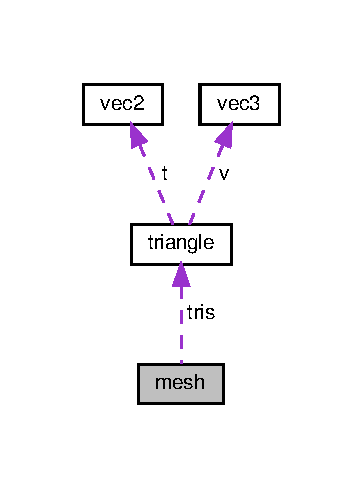
\includegraphics[width=174pt]{structmesh__coll__graph}
\end{center}
\end{figure}
\subsection*{Public Attributes}
\begin{DoxyCompactItemize}
\item 
\mbox{\Hypertarget{structmesh_a11dd56c45e9cb82c083ac3613c9cdadf}\label{structmesh_a11dd56c45e9cb82c083ac3613c9cdadf}} 
struct \hyperlink{structtriangle}{triangle} $\ast$ {\bfseries tris}
\item 
\mbox{\Hypertarget{structmesh_a1735083c139ec79acce73533f0b62be0}\label{structmesh_a1735083c139ec79acce73533f0b62be0}} 
int {\bfseries count}
\end{DoxyCompactItemize}


\subsection{Detailed Description}
A collection of triangles representing some kind of 3D model. 

The documentation for this struct was generated from the following file\+:\begin{DoxyCompactItemize}
\item 
\hyperlink{math_8h}{math.\+h}\end{DoxyCompactItemize}

\hypertarget{structtexture}{}\section{texture Struct Reference}
\label{structtexture}\index{texture@{texture}}


data is always R\+GB with 8-\/bits per component and no padding in rows.  




{\ttfamily \#include $<$texture.\+h$>$}

\subsection*{Public Attributes}
\begin{DoxyCompactItemize}
\item 
\mbox{\Hypertarget{structtexture_a1adde5ed6e5e51d7987713b9937c3a36}\label{structtexture_a1adde5ed6e5e51d7987713b9937c3a36}} 
unsigned char $\ast$ {\bfseries data}
\item 
\mbox{\Hypertarget{structtexture_a4a3a10c13e71ede50448d2206b19b3f0}\label{structtexture_a4a3a10c13e71ede50448d2206b19b3f0}} 
int {\bfseries width}
\item 
\mbox{\Hypertarget{structtexture_a349e2a1068e65f1520a4a4c0af28e28e}\label{structtexture_a349e2a1068e65f1520a4a4c0af28e28e}} 
int {\bfseries height}
\item 
\mbox{\Hypertarget{structtexture_ab7699885b4439c13cb908d43c9b27d38}\label{structtexture_ab7699885b4439c13cb908d43c9b27d38}} 
int {\bfseries num\+Bytes\+Per\+Pixel}
\end{DoxyCompactItemize}


\subsection{Detailed Description}
data is always R\+GB with 8-\/bits per component and no padding in rows. 

The documentation for this struct was generated from the following file\+:\begin{DoxyCompactItemize}
\item 
\hyperlink{texture_8h}{texture.\+h}\end{DoxyCompactItemize}

\hypertarget{structtriangle}{}\section{triangle Struct Reference}
\label{structtriangle}\index{triangle@{triangle}}


Triangular mesh face.  




{\ttfamily \#include $<$math.\+h$>$}



Collaboration diagram for triangle\+:\nopagebreak
\begin{figure}[H]
\begin{center}
\leavevmode
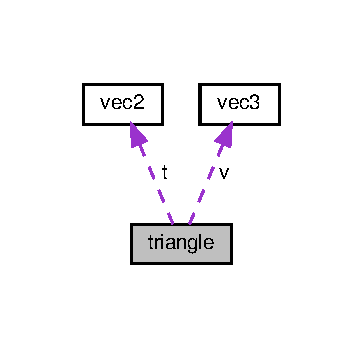
\includegraphics[width=174pt]{structtriangle__coll__graph}
\end{center}
\end{figure}
\subsection*{Public Attributes}
\begin{DoxyCompactItemize}
\item 
\mbox{\Hypertarget{structtriangle_a5bc62f2a81704e89e77d3b9b54c34be2}\label{structtriangle_a5bc62f2a81704e89e77d3b9b54c34be2}} 
\begin{tabbing}
xx\=xx\=xx\=xx\=xx\=xx\=xx\=xx\=xx\=\kill
union \{\\
\mbox{\Hypertarget{uniontriangle_1_1_0D8_a54d0d098812b0da9651917ea3402d139}\label{uniontriangle_1_1_0D8_a54d0d098812b0da9651917ea3402d139}} 
\>struct \{\\
\>\>float {\bfseries x1}\\
\>\>float {\bfseries y1}\\
\>\>float {\bfseries z1}\\
\>\>float {\bfseries w1}\\
\>\>float {\bfseries x2}\\
\>\>float {\bfseries y2}\\
\>\>float {\bfseries z2}\\
\>\>float {\bfseries w2}\\
\>\>float {\bfseries x3}\\
\>\>float {\bfseries y3}\\
\>\>float {\bfseries z3}\\
\>\>float {\bfseries w3}\\
\>\} \\
\>struct \hyperlink{structvec3}{vec3} {\bfseries v} \mbox{[}3\mbox{]}\\
\}; \\

\end{tabbing}\item 
\mbox{\Hypertarget{structtriangle_a21313e1a3507db1c3028ddb1bc186b28}\label{structtriangle_a21313e1a3507db1c3028ddb1bc186b28}} 
\begin{tabbing}
xx\=xx\=xx\=xx\=xx\=xx\=xx\=xx\=xx\=\kill
union \{\\
\mbox{\Hypertarget{uniontriangle_1_1_0D10_a12bac64045f3bf8e23abf4c84ba5110c}\label{uniontriangle_1_1_0D10_a12bac64045f3bf8e23abf4c84ba5110c}} 
\>struct \{\\
\>\>float {\bfseries u1}\\
\>\>float {\bfseries v1}\\
\>\>float {\bfseries tw1}\\
\>\>float {\bfseries u2}\\
\>\>float {\bfseries v2}\\
\>\>float {\bfseries tw2}\\
\>\>float {\bfseries u3}\\
\>\>float {\bfseries v3}\\
\>\>float {\bfseries tw3}\\
\>\} \\
\>struct \hyperlink{structvec2}{vec2} {\bfseries t} \mbox{[}3\mbox{]}\\
\}; \\

\end{tabbing}\item 
\mbox{\Hypertarget{structtriangle_a8e59a9188d073130c946f55f3d6f9955}\label{structtriangle_a8e59a9188d073130c946f55f3d6f9955}} 
unsigned int {\bfseries color}
\end{DoxyCompactItemize}


\subsection{Detailed Description}
Triangular mesh face. 

A mesh face consisting solely of homogenous 3D coordinates and homogenous 2D texture coordinates, and a color attribute.

Currently the color attribute is not used, but it is useful for debugging or falling back to in lieu of texture values or coordinate values. 

The documentation for this struct was generated from the following file\+:\begin{DoxyCompactItemize}
\item 
\hyperlink{math_8h}{math.\+h}\end{DoxyCompactItemize}

\hypertarget{structtriangle__list}{}\section{triangle\+\_\+list Struct Reference}
\label{structtriangle__list}\index{triangle\+\_\+list@{triangle\+\_\+list}}


Collaboration diagram for triangle\+\_\+list\+:\nopagebreak
\begin{figure}[H]
\begin{center}
\leavevmode
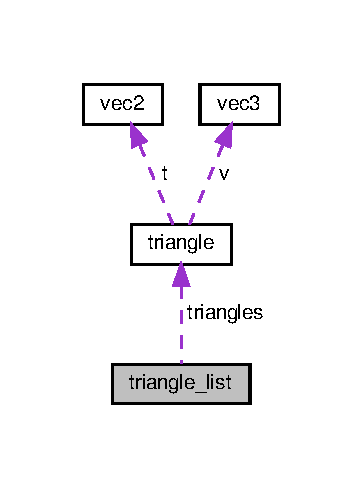
\includegraphics[width=174pt]{structtriangle__list__coll__graph}
\end{center}
\end{figure}
\subsection*{Public Attributes}
\begin{DoxyCompactItemize}
\item 
\mbox{\Hypertarget{structtriangle__list_a58b750d732071bd30a0befc681b69465}\label{structtriangle__list_a58b750d732071bd30a0befc681b69465}} 
struct \hyperlink{structtriangle}{triangle} {\bfseries triangles} \mbox{[}256\mbox{]}
\item 
\mbox{\Hypertarget{structtriangle__list_a207f63c76994dd2289372305653f6b69}\label{structtriangle__list_a207f63c76994dd2289372305653f6b69}} 
unsigned char {\bfseries head}
\item 
\mbox{\Hypertarget{structtriangle__list_aa5162192749bbef4c2776e236619b00b}\label{structtriangle__list_aa5162192749bbef4c2776e236619b00b}} 
unsigned char {\bfseries tail}
\end{DoxyCompactItemize}


The documentation for this struct was generated from the following file\+:\begin{DoxyCompactItemize}
\item 
\hyperlink{triangle__list_8h}{triangle\+\_\+list.\+h}\end{DoxyCompactItemize}

\hypertarget{structvec2}{}\section{vec2 Struct Reference}
\label{structvec2}\index{vec2@{vec2}}


Homogenous 2D coordinates.  




{\ttfamily \#include $<$math.\+h$>$}

\subsection*{Public Attributes}
\begin{DoxyCompactItemize}
\item 
\mbox{\Hypertarget{structvec2_adb6dab2d0bc861737c54dc7afa57225b}\label{structvec2_adb6dab2d0bc861737c54dc7afa57225b}} 
\begin{tabbing}
xx\=xx\=xx\=xx\=xx\=xx\=xx\=xx\=xx\=\kill
union \{\\
\mbox{\Hypertarget{unionvec2_1_1_0D0_aa6aeded6e4cc7a622b1049d41ca7c263}\label{unionvec2_1_1_0D0_aa6aeded6e4cc7a622b1049d41ca7c263}} 
\>struct \{\\
\>\>float {\bfseries u}\\
\>\>float {\bfseries v}\\
\>\>float {\bfseries w}\\
\>\} \\
\>float {\bfseries p} \mbox{[}3\mbox{]}\\
\}; \\

\end{tabbing}\end{DoxyCompactItemize}


\subsection{Detailed Description}
Homogenous 2D coordinates. 

A 3-\/element structure used to represent 2D coordinate space with 2 cartesian coordinates and a homogenous 3rd coordinate for projection. 

The documentation for this struct was generated from the following file\+:\begin{DoxyCompactItemize}
\item 
\hyperlink{math_8h}{math.\+h}\end{DoxyCompactItemize}

\hypertarget{structvec3}{}\section{vec3 Struct Reference}
\label{structvec3}\index{vec3@{vec3}}


Homogenous 3D coordinates.  




{\ttfamily \#include $<$math.\+h$>$}

\subsection*{Public Attributes}
\begin{DoxyCompactItemize}
\item 
\mbox{\Hypertarget{structvec3_ae5a1cf26166774918ebecc3a1c5cac4b}\label{structvec3_ae5a1cf26166774918ebecc3a1c5cac4b}} 
\begin{tabbing}
xx\=xx\=xx\=xx\=xx\=xx\=xx\=xx\=xx\=\kill
union \{\\
\mbox{\Hypertarget{unionvec3_1_1_0D4_a528169d018e689644b47b2222d1c9771}\label{unionvec3_1_1_0D4_a528169d018e689644b47b2222d1c9771}} 
\>struct \{\\
\>\>float {\bfseries x}\\
\>\>float {\bfseries y}\\
\>\>float {\bfseries z}\\
\>\>float {\bfseries w}\\
\>\} \\
\>float {\bfseries p} \mbox{[}4\mbox{]}\\
\}; \\

\end{tabbing}\end{DoxyCompactItemize}


\subsection{Detailed Description}
Homogenous 3D coordinates. 

A 4-\/element structure used to represent 3D coordinate space with 3 cartesian coordinates and a homogeouns 4th coordinate for projection. 

The documentation for this struct was generated from the following file\+:\begin{DoxyCompactItemize}
\item 
\hyperlink{math_8h}{math.\+h}\end{DoxyCompactItemize}

\chapter{File Documentation}
\hypertarget{color_8c}{}\section{color.\+c File Reference}
\label{color_8c}\index{color.\+c@{color.\+c}}
{\ttfamily \#include \char`\"{}color.\+h\char`\"{}}\newline
Include dependency graph for color.\+c\+:\nopagebreak
\begin{figure}[H]
\begin{center}
\leavevmode
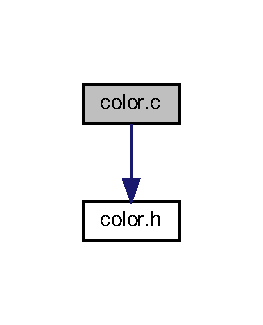
\includegraphics[width=126pt]{color_8c__incl}
\end{center}
\end{figure}
\subsection*{Functions}
\begin{DoxyCompactItemize}
\item 
void \hyperlink{color_8c_a1983b73905a47e4752ddaec3f4393f56}{Color\+Set\+Int} (struct \hyperlink{structcolor}{color} $\ast$\hyperlink{structcolor}{color}, char component, unsigned int value)
\begin{DoxyCompactList}\small\item\em Set the color component. \end{DoxyCompactList}\item 
void \hyperlink{color_8c_ade5db644fc75d29895e5ab029cc5ad73}{Color\+Set\+Float} (struct \hyperlink{structcolor}{color} $\ast$\hyperlink{structcolor}{color}, char component, float value)
\begin{DoxyCompactList}\small\item\em Set the color component. \end{DoxyCompactList}\item 
struct \hyperlink{structcolor}{color} \hyperlink{color_8c_a1d7333cef0f004aeb31626da38400230}{Color\+Init\+Float} (float r, float g, float b, float a)
\begin{DoxyCompactList}\small\item\em Initialize a new color with individual R, G, B, A components as floats. \end{DoxyCompactList}\item 
unsigned int \hyperlink{color_8c_adc8b67194c326a6c261a52121cf6c312}{Color\+Get\+Int} (struct \hyperlink{structcolor}{color} \hyperlink{structcolor}{color}, char component)
\begin{DoxyCompactList}\small\item\em Get the color component. \end{DoxyCompactList}\item 
float \hyperlink{color_8c_a5528f9c2a3d87e4612e1ce6cf8442bcf}{Color\+Get\+Float} (struct \hyperlink{structcolor}{color} \hyperlink{structcolor}{color}, char component)
\begin{DoxyCompactList}\small\item\em Get the color component. \end{DoxyCompactList}\end{DoxyCompactItemize}
\subsection*{Variables}
\begin{DoxyCompactItemize}
\item 
\mbox{\Hypertarget{color_8c_a46bbbca710bfede8eea3d1f3123d0b27}\label{color_8c_a46bbbca710bfede8eea3d1f3123d0b27}} 
struct \hyperlink{structcolor}{color} {\bfseries Color\+White} = \{ 0x\+F\+F\+F\+F\+F\+F\+F\+F \}
\item 
\mbox{\Hypertarget{color_8c_affde57444c7fbfb6e7522e6ce8eeaa4c}\label{color_8c_affde57444c7fbfb6e7522e6ce8eeaa4c}} 
struct \hyperlink{structcolor}{color} {\bfseries Color\+Black} = \{ 0x000000\+F\+F \}
\item 
\mbox{\Hypertarget{color_8c_ada36b5546b6d2ce9ac30a2ad9f1378fe}\label{color_8c_ada36b5546b6d2ce9ac30a2ad9f1378fe}} 
struct \hyperlink{structcolor}{color} {\bfseries Color\+Red} = \{ 0x\+F\+F0000\+F\+F \}
\item 
\mbox{\Hypertarget{color_8c_a5a7b6855f667940f9171700200bf8898}\label{color_8c_a5a7b6855f667940f9171700200bf8898}} 
struct \hyperlink{structcolor}{color} {\bfseries Color\+Green} = \{ 0x00\+F\+F00\+F\+F \}
\item 
\mbox{\Hypertarget{color_8c_a6e67b5067389be109d1914035a91d130}\label{color_8c_a6e67b5067389be109d1914035a91d130}} 
struct \hyperlink{structcolor}{color} {\bfseries Color\+Blue} = \{ 0x0000\+F\+F\+F\+F \}
\item 
\mbox{\Hypertarget{color_8c_ab6df53354e9db2fc69aadebd0b83469a}\label{color_8c_ab6df53354e9db2fc69aadebd0b83469a}} 
struct \hyperlink{structcolor}{color} {\bfseries Color\+Purple} = \{ 0x7\+F00\+F\+F\+F\+F \}
\item 
\mbox{\Hypertarget{color_8c_a7b09b6d4d453d24000a2f3ca65bc2e32}\label{color_8c_a7b09b6d4d453d24000a2f3ca65bc2e32}} 
struct \hyperlink{structcolor}{color} {\bfseries Color\+Yellow} = \{ 0x\+F\+F\+F\+F00\+F\+F \}
\item 
\mbox{\Hypertarget{color_8c_a5f3c7f8b2abbe2523b52195ff5f674d8}\label{color_8c_a5f3c7f8b2abbe2523b52195ff5f674d8}} 
struct \hyperlink{structcolor}{color} {\bfseries Color\+Cyan} = \{ 0x00\+F\+F\+F\+F\+F\+F \}
\item 
\mbox{\Hypertarget{color_8c_a5428590e2be17762f29ff260205cd8b5}\label{color_8c_a5428590e2be17762f29ff260205cd8b5}} 
struct \hyperlink{structcolor}{color} {\bfseries Color\+Pink} = \{ 0x\+F\+F00\+F\+F\+F\+F \}
\end{DoxyCompactItemize}


\subsection{Function Documentation}
\mbox{\Hypertarget{color_8c_a5528f9c2a3d87e4612e1ce6cf8442bcf}\label{color_8c_a5528f9c2a3d87e4612e1ce6cf8442bcf}} 
\index{color.\+c@{color.\+c}!Color\+Get\+Float@{Color\+Get\+Float}}
\index{Color\+Get\+Float@{Color\+Get\+Float}!color.\+c@{color.\+c}}
\subsubsection{\texorpdfstring{Color\+Get\+Float()}{ColorGetFloat()}}
{\footnotesize\ttfamily float Color\+Get\+Float (\begin{DoxyParamCaption}\item[{struct \hyperlink{structcolor}{color}}]{color,  }\item[{char}]{component }\end{DoxyParamCaption})}



Get the color component. 

The component is returned as a float in the range \mbox{[}0.\+0,1.\+0\mbox{]}


\begin{DoxyParams}{Parameters}
{\em color} & color object to read \\
\hline
{\em component} & \textquotesingle{}r\textquotesingle{}, \textquotesingle{}g\textquotesingle{}, \textquotesingle{}b\textquotesingle{} or \textquotesingle{}a\textquotesingle{} exclusively. \\
\hline
\end{DoxyParams}
\begin{DoxyReturn}{Returns}
value of the color component 
\end{DoxyReturn}
\mbox{\Hypertarget{color_8c_adc8b67194c326a6c261a52121cf6c312}\label{color_8c_adc8b67194c326a6c261a52121cf6c312}} 
\index{color.\+c@{color.\+c}!Color\+Get\+Int@{Color\+Get\+Int}}
\index{Color\+Get\+Int@{Color\+Get\+Int}!color.\+c@{color.\+c}}
\subsubsection{\texorpdfstring{Color\+Get\+Int()}{ColorGetInt()}}
{\footnotesize\ttfamily unsigned int Color\+Get\+Int (\begin{DoxyParamCaption}\item[{struct \hyperlink{structcolor}{color}}]{color,  }\item[{char}]{component }\end{DoxyParamCaption})}



Get the color component. 

The component is returned as the raw integer value, in the range \mbox{[}0,255\mbox{]}


\begin{DoxyParams}{Parameters}
{\em color} & color object to read \\
\hline
{\em component} & \textquotesingle{}r\textquotesingle{}, \textquotesingle{}g\textquotesingle{}, \textquotesingle{}b\textquotesingle{} or \textquotesingle{}a\textquotesingle{} exclusively. \\
\hline
\end{DoxyParams}
\begin{DoxyReturn}{Returns}
value of the color component 
\end{DoxyReturn}
\mbox{\Hypertarget{color_8c_a1d7333cef0f004aeb31626da38400230}\label{color_8c_a1d7333cef0f004aeb31626da38400230}} 
\index{color.\+c@{color.\+c}!Color\+Init\+Float@{Color\+Init\+Float}}
\index{Color\+Init\+Float@{Color\+Init\+Float}!color.\+c@{color.\+c}}
\subsubsection{\texorpdfstring{Color\+Init\+Float()}{ColorInitFloat()}}
{\footnotesize\ttfamily struct \hyperlink{structcolor}{color} Color\+Init\+Float (\begin{DoxyParamCaption}\item[{float}]{r,  }\item[{float}]{g,  }\item[{float}]{b,  }\item[{float}]{a }\end{DoxyParamCaption})}



Initialize a new color with individual R, G, B, A components as floats. 


\begin{DoxyParams}{Parameters}
{\em r} & Red component from 0 to 1 \\
\hline
{\em g} & Green componenet from 0 to 1 \\
\hline
{\em b} & Blue component from 0 to 1 \\
\hline
{\em a} & Alpha component, from 0 to 1 \\
\hline
\end{DoxyParams}
\begin{DoxyReturn}{Returns}
resulting color object 
\end{DoxyReturn}
\mbox{\Hypertarget{color_8c_ade5db644fc75d29895e5ab029cc5ad73}\label{color_8c_ade5db644fc75d29895e5ab029cc5ad73}} 
\index{color.\+c@{color.\+c}!Color\+Set\+Float@{Color\+Set\+Float}}
\index{Color\+Set\+Float@{Color\+Set\+Float}!color.\+c@{color.\+c}}
\subsubsection{\texorpdfstring{Color\+Set\+Float()}{ColorSetFloat()}}
{\footnotesize\ttfamily void Color\+Set\+Float (\begin{DoxyParamCaption}\item[{struct \hyperlink{structcolor}{color} $\ast$}]{color,  }\item[{char}]{component,  }\item[{float}]{value }\end{DoxyParamCaption})}



Set the color component. 

The value should be a float in the range \mbox{[}0.\+0,1.\+0\mbox{]}


\begin{DoxyParams}{Parameters}
{\em color} & pointer to the color object to write \\
\hline
{\em component} & \textquotesingle{}r\textquotesingle{}, \textquotesingle{}g\textquotesingle{}, \textquotesingle{}b\textquotesingle{} or \textquotesingle{}a\textquotesingle{} exclusively. \\
\hline
{\em value} & value of the color component to set \\
\hline
\end{DoxyParams}
\mbox{\Hypertarget{color_8c_a1983b73905a47e4752ddaec3f4393f56}\label{color_8c_a1983b73905a47e4752ddaec3f4393f56}} 
\index{color.\+c@{color.\+c}!Color\+Set\+Int@{Color\+Set\+Int}}
\index{Color\+Set\+Int@{Color\+Set\+Int}!color.\+c@{color.\+c}}
\subsubsection{\texorpdfstring{Color\+Set\+Int()}{ColorSetInt()}}
{\footnotesize\ttfamily void Color\+Set\+Int (\begin{DoxyParamCaption}\item[{struct \hyperlink{structcolor}{color} $\ast$}]{color,  }\item[{char}]{component,  }\item[{unsigned int}]{value }\end{DoxyParamCaption})}



Set the color component. 

The value should be an integer in the range \mbox{[}0,255\mbox{]}


\begin{DoxyParams}{Parameters}
{\em color} & pointer to the color object to write \\
\hline
{\em component} & \textquotesingle{}r\textquotesingle{}, \textquotesingle{}g\textquotesingle{}, \textquotesingle{}b\textquotesingle{} or \textquotesingle{}a\textquotesingle{} exclusively. \\
\hline
{\em value} & value of the color component to set \\
\hline
\end{DoxyParams}

\hypertarget{color_8h}{}\section{color.\+h File Reference}
\label{color_8h}\index{color.\+h@{color.\+h}}
This graph shows which files directly or indirectly include this file\+:\nopagebreak
\begin{figure}[H]
\begin{center}
\leavevmode
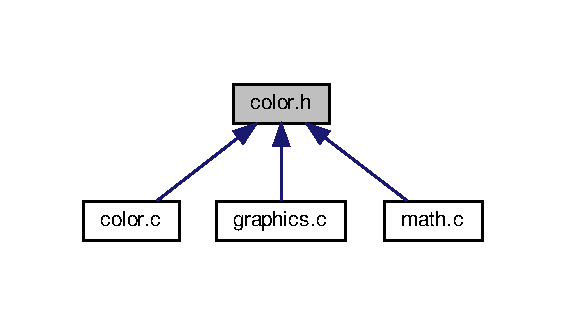
\includegraphics[width=272pt]{color_8h__dep__incl}
\end{center}
\end{figure}
\subsection*{Classes}
\begin{DoxyCompactItemize}
\item 
struct \hyperlink{structcolor}{color}
\begin{DoxyCompactList}\small\item\em R\+G\+BA color quad. \end{DoxyCompactList}\end{DoxyCompactItemize}
\subsection*{Macros}
\begin{DoxyCompactItemize}
\item 
\mbox{\Hypertarget{color_8h_aad1216fd05e1ecf7d77aaa540cce6ba0}\label{color_8h_aad1216fd05e1ecf7d77aaa540cce6ba0}} 
\#define \hyperlink{color_8h_aad1216fd05e1ecf7d77aaa540cce6ba0}{C\+O\+L\+O\+R\+\_\+\+V\+E\+R\+S\+I\+ON}~\char`\"{}0.\+1.\+0\char`\"{}
\begin{DoxyCompactList}\small\item\em include guard \end{DoxyCompactList}\end{DoxyCompactItemize}
\subsection*{Functions}
\begin{DoxyCompactItemize}
\item 
struct \hyperlink{structcolor}{color} \hyperlink{color_8h_a1d7333cef0f004aeb31626da38400230}{Color\+Init\+Float} (float r, float g, float b, float a)
\begin{DoxyCompactList}\small\item\em Initialize a new color with individual R, G, B, A components as floats. \end{DoxyCompactList}\item 
unsigned int \hyperlink{color_8h_adc8b67194c326a6c261a52121cf6c312}{Color\+Get\+Int} (struct \hyperlink{structcolor}{color} \hyperlink{structcolor}{color}, char component)
\begin{DoxyCompactList}\small\item\em Get the color component. \end{DoxyCompactList}\item 
float \hyperlink{color_8h_a5528f9c2a3d87e4612e1ce6cf8442bcf}{Color\+Get\+Float} (struct \hyperlink{structcolor}{color} \hyperlink{structcolor}{color}, char component)
\begin{DoxyCompactList}\small\item\em Get the color component. \end{DoxyCompactList}\item 
void \hyperlink{color_8h_a1983b73905a47e4752ddaec3f4393f56}{Color\+Set\+Int} (struct \hyperlink{structcolor}{color} $\ast$\hyperlink{structcolor}{color}, char component, unsigned int value)
\begin{DoxyCompactList}\small\item\em Set the color component. \end{DoxyCompactList}\item 
void \hyperlink{color_8h_ade5db644fc75d29895e5ab029cc5ad73}{Color\+Set\+Float} (struct \hyperlink{structcolor}{color} $\ast$\hyperlink{structcolor}{color}, char component, float value)
\begin{DoxyCompactList}\small\item\em Set the color component. \end{DoxyCompactList}\end{DoxyCompactItemize}
\subsection*{Variables}
\begin{DoxyCompactItemize}
\item 
\mbox{\Hypertarget{color_8h_a46bbbca710bfede8eea3d1f3123d0b27}\label{color_8h_a46bbbca710bfede8eea3d1f3123d0b27}} 
struct \hyperlink{structcolor}{color} {\bfseries Color\+White}
\item 
\mbox{\Hypertarget{color_8h_affde57444c7fbfb6e7522e6ce8eeaa4c}\label{color_8h_affde57444c7fbfb6e7522e6ce8eeaa4c}} 
struct \hyperlink{structcolor}{color} {\bfseries Color\+Black}
\item 
\mbox{\Hypertarget{color_8h_ada36b5546b6d2ce9ac30a2ad9f1378fe}\label{color_8h_ada36b5546b6d2ce9ac30a2ad9f1378fe}} 
struct \hyperlink{structcolor}{color} {\bfseries Color\+Red}
\item 
\mbox{\Hypertarget{color_8h_a5a7b6855f667940f9171700200bf8898}\label{color_8h_a5a7b6855f667940f9171700200bf8898}} 
struct \hyperlink{structcolor}{color} {\bfseries Color\+Green}
\item 
\mbox{\Hypertarget{color_8h_a6e67b5067389be109d1914035a91d130}\label{color_8h_a6e67b5067389be109d1914035a91d130}} 
struct \hyperlink{structcolor}{color} {\bfseries Color\+Blue}
\item 
\mbox{\Hypertarget{color_8h_ab6df53354e9db2fc69aadebd0b83469a}\label{color_8h_ab6df53354e9db2fc69aadebd0b83469a}} 
struct \hyperlink{structcolor}{color} {\bfseries Color\+Purple}
\item 
\mbox{\Hypertarget{color_8h_a7b09b6d4d453d24000a2f3ca65bc2e32}\label{color_8h_a7b09b6d4d453d24000a2f3ca65bc2e32}} 
struct \hyperlink{structcolor}{color} {\bfseries Color\+Yellow}
\item 
\mbox{\Hypertarget{color_8h_a5f3c7f8b2abbe2523b52195ff5f674d8}\label{color_8h_a5f3c7f8b2abbe2523b52195ff5f674d8}} 
struct \hyperlink{structcolor}{color} {\bfseries Color\+Cyan}
\item 
\mbox{\Hypertarget{color_8h_a5428590e2be17762f29ff260205cd8b5}\label{color_8h_a5428590e2be17762f29ff260205cd8b5}} 
struct \hyperlink{structcolor}{color} {\bfseries Color\+Pink}
\end{DoxyCompactItemize}


\subsection{Detailed Description}
This interface attempts to provide an intuitive wrapper around \char`\"{}raw\char`\"{} unsigned integer colors.

An unsigned integer color is packed 32-\/bit value consisting of 4 pixel elements\+: R\+G\+BA. These elements are stored as written\+: R\+G\+BA, or, visually mapped as hex symbols\+: R\+R\+G\+G\+B\+B\+AA. 

\subsection{Function Documentation}
\mbox{\Hypertarget{color_8h_a5528f9c2a3d87e4612e1ce6cf8442bcf}\label{color_8h_a5528f9c2a3d87e4612e1ce6cf8442bcf}} 
\index{color.\+h@{color.\+h}!Color\+Get\+Float@{Color\+Get\+Float}}
\index{Color\+Get\+Float@{Color\+Get\+Float}!color.\+h@{color.\+h}}
\subsubsection{\texorpdfstring{Color\+Get\+Float()}{ColorGetFloat()}}
{\footnotesize\ttfamily float Color\+Get\+Float (\begin{DoxyParamCaption}\item[{struct \hyperlink{structcolor}{color}}]{color,  }\item[{char}]{component }\end{DoxyParamCaption})}



Get the color component. 

The component is returned as a float in the range \mbox{[}0.\+0,1.\+0\mbox{]}


\begin{DoxyParams}{Parameters}
{\em color} & color object to read \\
\hline
{\em component} & \textquotesingle{}r\textquotesingle{}, \textquotesingle{}g\textquotesingle{}, \textquotesingle{}b\textquotesingle{} or \textquotesingle{}a\textquotesingle{} exclusively. \\
\hline
\end{DoxyParams}
\begin{DoxyReturn}{Returns}
value of the color component 
\end{DoxyReturn}
\mbox{\Hypertarget{color_8h_adc8b67194c326a6c261a52121cf6c312}\label{color_8h_adc8b67194c326a6c261a52121cf6c312}} 
\index{color.\+h@{color.\+h}!Color\+Get\+Int@{Color\+Get\+Int}}
\index{Color\+Get\+Int@{Color\+Get\+Int}!color.\+h@{color.\+h}}
\subsubsection{\texorpdfstring{Color\+Get\+Int()}{ColorGetInt()}}
{\footnotesize\ttfamily unsigned int Color\+Get\+Int (\begin{DoxyParamCaption}\item[{struct \hyperlink{structcolor}{color}}]{color,  }\item[{char}]{component }\end{DoxyParamCaption})}



Get the color component. 

The component is returned as the raw integer value, in the range \mbox{[}0,255\mbox{]}


\begin{DoxyParams}{Parameters}
{\em color} & color object to read \\
\hline
{\em component} & \textquotesingle{}r\textquotesingle{}, \textquotesingle{}g\textquotesingle{}, \textquotesingle{}b\textquotesingle{} or \textquotesingle{}a\textquotesingle{} exclusively. \\
\hline
\end{DoxyParams}
\begin{DoxyReturn}{Returns}
value of the color component 
\end{DoxyReturn}
\mbox{\Hypertarget{color_8h_a1d7333cef0f004aeb31626da38400230}\label{color_8h_a1d7333cef0f004aeb31626da38400230}} 
\index{color.\+h@{color.\+h}!Color\+Init\+Float@{Color\+Init\+Float}}
\index{Color\+Init\+Float@{Color\+Init\+Float}!color.\+h@{color.\+h}}
\subsubsection{\texorpdfstring{Color\+Init\+Float()}{ColorInitFloat()}}
{\footnotesize\ttfamily struct \hyperlink{structcolor}{color} Color\+Init\+Float (\begin{DoxyParamCaption}\item[{float}]{r,  }\item[{float}]{g,  }\item[{float}]{b,  }\item[{float}]{a }\end{DoxyParamCaption})}



Initialize a new color with individual R, G, B, A components as floats. 


\begin{DoxyParams}{Parameters}
{\em r} & Red component from 0 to 1 \\
\hline
{\em g} & Green componenet from 0 to 1 \\
\hline
{\em b} & Blue component from 0 to 1 \\
\hline
{\em a} & Alpha component, from 0 to 1 \\
\hline
\end{DoxyParams}
\begin{DoxyReturn}{Returns}
resulting color object 
\end{DoxyReturn}
\mbox{\Hypertarget{color_8h_ade5db644fc75d29895e5ab029cc5ad73}\label{color_8h_ade5db644fc75d29895e5ab029cc5ad73}} 
\index{color.\+h@{color.\+h}!Color\+Set\+Float@{Color\+Set\+Float}}
\index{Color\+Set\+Float@{Color\+Set\+Float}!color.\+h@{color.\+h}}
\subsubsection{\texorpdfstring{Color\+Set\+Float()}{ColorSetFloat()}}
{\footnotesize\ttfamily void Color\+Set\+Float (\begin{DoxyParamCaption}\item[{struct \hyperlink{structcolor}{color} $\ast$}]{color,  }\item[{char}]{component,  }\item[{float}]{value }\end{DoxyParamCaption})}



Set the color component. 

The value should be a float in the range \mbox{[}0.\+0,1.\+0\mbox{]}


\begin{DoxyParams}{Parameters}
{\em color} & pointer to the color object to write \\
\hline
{\em component} & \textquotesingle{}r\textquotesingle{}, \textquotesingle{}g\textquotesingle{}, \textquotesingle{}b\textquotesingle{} or \textquotesingle{}a\textquotesingle{} exclusively. \\
\hline
{\em value} & value of the color component to set \\
\hline
\end{DoxyParams}
\mbox{\Hypertarget{color_8h_a1983b73905a47e4752ddaec3f4393f56}\label{color_8h_a1983b73905a47e4752ddaec3f4393f56}} 
\index{color.\+h@{color.\+h}!Color\+Set\+Int@{Color\+Set\+Int}}
\index{Color\+Set\+Int@{Color\+Set\+Int}!color.\+h@{color.\+h}}
\subsubsection{\texorpdfstring{Color\+Set\+Int()}{ColorSetInt()}}
{\footnotesize\ttfamily void Color\+Set\+Int (\begin{DoxyParamCaption}\item[{struct \hyperlink{structcolor}{color} $\ast$}]{color,  }\item[{char}]{component,  }\item[{unsigned int}]{value }\end{DoxyParamCaption})}



Set the color component. 

The value should be an integer in the range \mbox{[}0,255\mbox{]}


\begin{DoxyParams}{Parameters}
{\em color} & pointer to the color object to write \\
\hline
{\em component} & \textquotesingle{}r\textquotesingle{}, \textquotesingle{}g\textquotesingle{}, \textquotesingle{}b\textquotesingle{} or \textquotesingle{}a\textquotesingle{} exclusively. \\
\hline
{\em value} & value of the color component to set \\
\hline
\end{DoxyParams}

\hypertarget{graphics_8c}{}\section{graphics.\+c File Reference}
\label{graphics_8c}\index{graphics.\+c@{graphics.\+c}}
{\ttfamily \#include $<$string.\+h$>$}\newline
{\ttfamily \#include $<$stdio.\+h$>$}\newline
{\ttfamily \#include \char`\"{}S\+D\+L2/\+S\+D\+L.\+h\char`\"{}}\newline
{\ttfamily \#include \char`\"{}math.\+h\char`\"{}}\newline
{\ttfamily \#include \char`\"{}graphics.\+h\char`\"{}}\newline
{\ttfamily \#include \char`\"{}texture.\+h\char`\"{}}\newline
{\ttfamily \#include \char`\"{}color.\+h\char`\"{}}\newline
Include dependency graph for graphics.\+c\+:\nopagebreak
\begin{figure}[H]
\begin{center}
\leavevmode
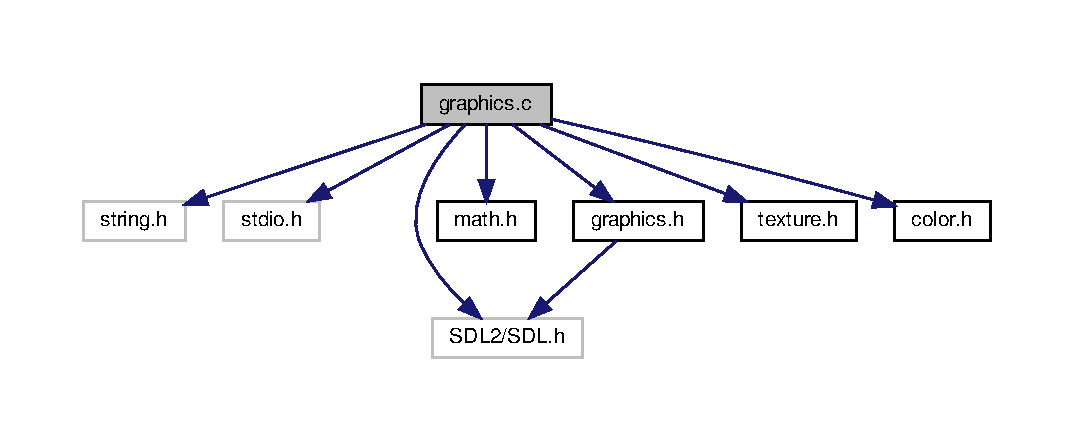
\includegraphics[width=350pt]{graphics_8c__incl}
\end{center}
\end{figure}
\subsection*{Classes}
\begin{DoxyCompactItemize}
\item 
struct \hyperlink{structgraphics}{graphics}
\begin{DoxyCompactList}\small\item\em Graphics state. \end{DoxyCompactList}\end{DoxyCompactItemize}
\subsection*{Functions}
\begin{DoxyCompactItemize}
\item 
void \hyperlink{graphics_8c_af5d2cafafbdf2ae4999226d24482303d}{swap\+\_\+generic} (void $\ast$v1, void $\ast$v2, size\+\_\+t size)
\begin{DoxyCompactList}\small\item\em A mostly generic implementation of swap. \end{DoxyCompactList}\item 
struct \hyperlink{structgraphics}{graphics} $\ast$ \hyperlink{graphics_8c_a543e265f9ff924a1def601674c56b3a2}{Graphics\+Init} (char $\ast$title, int width, int height, int scale)
\begin{DoxyCompactList}\small\item\em Creates and initializes a new graphics object isntance. \end{DoxyCompactList}\item 
void \hyperlink{graphics_8c_af08b9bb21695971ccac333eb31bc76ec}{Graphics\+Deinit} (struct \hyperlink{structgraphics}{graphics} $\ast$g)
\begin{DoxyCompactList}\small\item\em De-\/initializes and frees memory for the given graphics object. \end{DoxyCompactList}\item 
void \hyperlink{graphics_8c_acc8d5ed3b6d471a3df71f6c080f57194}{Graphics\+Begin} (struct \hyperlink{structgraphics}{graphics} $\ast$\hyperlink{structgraphics}{graphics})
\begin{DoxyCompactList}\small\item\em Initializes the graphics subsystem for drawing routines. \end{DoxyCompactList}\item 
void \hyperlink{graphics_8c_a93d049610e6a7de779502b748fe0a84a}{Graphics\+End} (struct \hyperlink{structgraphics}{graphics} $\ast$\hyperlink{structgraphics}{graphics})
\begin{DoxyCompactList}\small\item\em Prepares the graphics subsystem for presentation, then presents. \end{DoxyCompactList}\item 
void \hyperlink{graphics_8c_ac7cff8334dd93066be5801a7a12b00df}{Graphics\+Clear\+Screen} (struct \hyperlink{structgraphics}{graphics} $\ast$\hyperlink{structgraphics}{graphics}, unsigned int \hyperlink{structcolor}{color})
\begin{DoxyCompactList}\small\item\em Sets all pixels in the screen to the given color. \end{DoxyCompactList}\item 
void \hyperlink{graphics_8c_a80d44b851e06c1056dbd7aa765f95867}{Put\+Pixel\+Scaled} (struct \hyperlink{structgraphics}{graphics} $\ast$\hyperlink{structgraphics}{graphics}, int x, int y, unsigned int \hyperlink{structcolor}{color})
\begin{DoxyCompactList}\small\item\em Scale the pixel being drawn. \end{DoxyCompactList}\item 
void \hyperlink{graphics_8c_a577c98b0e997ec6a7a394f72e60968f7}{Put\+Pixel} (struct \hyperlink{structgraphics}{graphics} $\ast$\hyperlink{structgraphics}{graphics}, int x, int y, unsigned int \hyperlink{structcolor}{color})
\begin{DoxyCompactList}\small\item\em Put a pixel into the graphics buffer. \end{DoxyCompactList}\item 
void \hyperlink{graphics_8c_af9bdbd7f56505bc352579153c04f1051}{Graphics\+Draw\+Line} (struct \hyperlink{structgraphics}{graphics} $\ast$\hyperlink{structgraphics}{graphics}, int x1, int y1, int x2, int y2, unsigned int \hyperlink{structcolor}{color})
\begin{DoxyCompactList}\small\item\em Draws a line from (x1,y1) to (x2,y2) \end{DoxyCompactList}\item 
void \hyperlink{graphics_8c_a50ea5ae7900c76984aa7beabaa79532b}{Graphics\+Triangle\+Textured} (struct \hyperlink{structgraphics}{graphics} $\ast$\hyperlink{structgraphics}{graphics}, struct \hyperlink{structtriangle}{triangle} tri, struct \hyperlink{structtexture}{texture} $\ast$\hyperlink{structtexture}{texture})
\begin{DoxyCompactList}\small\item\em Draw a textured triangle with the given set of x and y coordinates. \end{DoxyCompactList}\item 
void \hyperlink{graphics_8c_ab4eed4462ddf5c15ca6ee40500850f5f}{Graphics\+Triangle\+Wireframe} (struct \hyperlink{structgraphics}{graphics} $\ast$\hyperlink{structgraphics}{graphics}, struct \hyperlink{structtriangle}{triangle} \hyperlink{structtriangle}{triangle}, unsigned int \hyperlink{structcolor}{color})
\begin{DoxyCompactList}\small\item\em Draw a triangle with the given set of x and y coordinates. \end{DoxyCompactList}\item 
\mbox{\Hypertarget{graphics_8c_a1c0c231b466914b51781b0908836e682}\label{graphics_8c_a1c0c231b466914b51781b0908836e682}} 
void \hyperlink{graphics_8c_a1c0c231b466914b51781b0908836e682}{Triangle\+Solid\+Draw\+Line} (struct \hyperlink{structgraphics}{graphics} $\ast$\hyperlink{structgraphics}{graphics}, int xmin, int xmax, int y, unsigned int \hyperlink{structcolor}{color})
\begin{DoxyCompactList}\small\item\em Used internally by \hyperlink{graphics_8c_a0ced2380f07dd02a2251f70480c8a0a9}{Graphics\+Triangle\+Solid()} \end{DoxyCompactList}\item 
void \hyperlink{graphics_8c_a0ced2380f07dd02a2251f70480c8a0a9}{Graphics\+Triangle\+Solid} (struct \hyperlink{structgraphics}{graphics} $\ast$\hyperlink{structgraphics}{graphics}, struct \hyperlink{structtriangle}{triangle} \hyperlink{structtriangle}{triangle}, unsigned int \hyperlink{structcolor}{color})
\begin{DoxyCompactList}\small\item\em Draw a triangle with the given set of x and y coordinates. \end{DoxyCompactList}\end{DoxyCompactItemize}


\subsection{Function Documentation}
\mbox{\Hypertarget{graphics_8c_acc8d5ed3b6d471a3df71f6c080f57194}\label{graphics_8c_acc8d5ed3b6d471a3df71f6c080f57194}} 
\index{graphics.\+c@{graphics.\+c}!Graphics\+Begin@{Graphics\+Begin}}
\index{Graphics\+Begin@{Graphics\+Begin}!graphics.\+c@{graphics.\+c}}
\subsubsection{\texorpdfstring{Graphics\+Begin()}{GraphicsBegin()}}
{\footnotesize\ttfamily void Graphics\+Begin (\begin{DoxyParamCaption}\item[{struct \hyperlink{structgraphics}{graphics} $\ast$}]{graphics }\end{DoxyParamCaption})}



Initializes the graphics subsystem for drawing routines. 

Internally locks streaming texture for direct manipulation.


\begin{DoxyParams}[1]{Parameters}
\mbox{\tt in,out}  & {\em graphics} & Graphics state to be manipulated \\
\hline
\end{DoxyParams}
\mbox{\Hypertarget{graphics_8c_ac7cff8334dd93066be5801a7a12b00df}\label{graphics_8c_ac7cff8334dd93066be5801a7a12b00df}} 
\index{graphics.\+c@{graphics.\+c}!Graphics\+Clear\+Screen@{Graphics\+Clear\+Screen}}
\index{Graphics\+Clear\+Screen@{Graphics\+Clear\+Screen}!graphics.\+c@{graphics.\+c}}
\subsubsection{\texorpdfstring{Graphics\+Clear\+Screen()}{GraphicsClearScreen()}}
{\footnotesize\ttfamily void Graphics\+Clear\+Screen (\begin{DoxyParamCaption}\item[{struct \hyperlink{structgraphics}{graphics} $\ast$}]{graphics,  }\item[{unsigned int}]{color }\end{DoxyParamCaption})}



Sets all pixels in the screen to the given color. 


\begin{DoxyParams}[1]{Parameters}
\mbox{\tt in,out}  & {\em graphics} & Graphics state to be manipulated \\
\hline
\mbox{\tt in}  & {\em color} & 32-\/bit color with 8-\/bits per component\+: (R,G,B,A) \\
\hline
\end{DoxyParams}
\mbox{\Hypertarget{graphics_8c_af08b9bb21695971ccac333eb31bc76ec}\label{graphics_8c_af08b9bb21695971ccac333eb31bc76ec}} 
\index{graphics.\+c@{graphics.\+c}!Graphics\+Deinit@{Graphics\+Deinit}}
\index{Graphics\+Deinit@{Graphics\+Deinit}!graphics.\+c@{graphics.\+c}}
\subsubsection{\texorpdfstring{Graphics\+Deinit()}{GraphicsDeinit()}}
{\footnotesize\ttfamily void Graphics\+Deinit (\begin{DoxyParamCaption}\item[{struct \hyperlink{structgraphics}{graphics} $\ast$}]{graphics }\end{DoxyParamCaption})}



De-\/initializes and frees memory for the given graphics object. 


\begin{DoxyParams}[1]{Parameters}
\mbox{\tt in,out}  & {\em graphics} & The initialized opcode object to be cleaned and reclaimed \\
\hline
\end{DoxyParams}
\mbox{\Hypertarget{graphics_8c_af9bdbd7f56505bc352579153c04f1051}\label{graphics_8c_af9bdbd7f56505bc352579153c04f1051}} 
\index{graphics.\+c@{graphics.\+c}!Graphics\+Draw\+Line@{Graphics\+Draw\+Line}}
\index{Graphics\+Draw\+Line@{Graphics\+Draw\+Line}!graphics.\+c@{graphics.\+c}}
\subsubsection{\texorpdfstring{Graphics\+Draw\+Line()}{GraphicsDrawLine()}}
{\footnotesize\ttfamily void Graphics\+Draw\+Line (\begin{DoxyParamCaption}\item[{struct \hyperlink{structgraphics}{graphics} $\ast$}]{graphics,  }\item[{int}]{x1,  }\item[{int}]{y1,  }\item[{int}]{x2,  }\item[{int}]{y2,  }\item[{unsigned int}]{color }\end{DoxyParamCaption})}



Draws a line from (x1,y1) to (x2,y2) 

Used by \hyperlink{graphics_8c_ab4eed4462ddf5c15ca6ee40500850f5f}{Graphics\+Triangle\+Wireframe()} and \hyperlink{graphics_8c_a0ced2380f07dd02a2251f70480c8a0a9}{Graphics\+Triangle\+Solid()}


\begin{DoxyParams}[1]{Parameters}
\mbox{\tt in,out}  & {\em graphics} & Graphics state to be manipulated \\
\hline
\mbox{\tt in}  & {\em x1} & horizontal position of the line start. \\
\hline
\mbox{\tt in}  & {\em y1} & vertical position of the line start. \\
\hline
\mbox{\tt in}  & {\em x2} & horizontal position of the line end. \\
\hline
\mbox{\tt in}  & {\em y2} & vertical position of the line end. \\
\hline
\mbox{\tt in}  & {\em color} & color to render the line with. \\
\hline
\end{DoxyParams}
\mbox{\Hypertarget{graphics_8c_a93d049610e6a7de779502b748fe0a84a}\label{graphics_8c_a93d049610e6a7de779502b748fe0a84a}} 
\index{graphics.\+c@{graphics.\+c}!Graphics\+End@{Graphics\+End}}
\index{Graphics\+End@{Graphics\+End}!graphics.\+c@{graphics.\+c}}
\subsubsection{\texorpdfstring{Graphics\+End()}{GraphicsEnd()}}
{\footnotesize\ttfamily void Graphics\+End (\begin{DoxyParamCaption}\item[{struct \hyperlink{structgraphics}{graphics} $\ast$}]{graphics }\end{DoxyParamCaption})}



Prepares the graphics subsystem for presentation, then presents. 

Internally unlocks streaming texture then calls presentation routines.


\begin{DoxyParams}[1]{Parameters}
\mbox{\tt in,out}  & {\em graphics} & Graphics state to be manipulated. \\
\hline
\end{DoxyParams}
\mbox{\Hypertarget{graphics_8c_a543e265f9ff924a1def601674c56b3a2}\label{graphics_8c_a543e265f9ff924a1def601674c56b3a2}} 
\index{graphics.\+c@{graphics.\+c}!Graphics\+Init@{Graphics\+Init}}
\index{Graphics\+Init@{Graphics\+Init}!graphics.\+c@{graphics.\+c}}
\subsubsection{\texorpdfstring{Graphics\+Init()}{GraphicsInit()}}
{\footnotesize\ttfamily struct \hyperlink{structgraphics}{graphics}$\ast$ Graphics\+Init (\begin{DoxyParamCaption}\item[{char $\ast$}]{title,  }\item[{int}]{width,  }\item[{int}]{height,  }\item[{int}]{scale }\end{DoxyParamCaption})}



Creates and initializes a new graphics object isntance. 

Scale can be specified as a non-\/negative number. This value is used to multiply both the width and the height and the pixel size of any drawing operations.

For example, specifying a scale of 2 would multiply the width by 2, the height by 2, and every pixel would be 2x2; so the total scale factor ends up being scale$^\wedge$2


\begin{DoxyParams}[1]{Parameters}
\mbox{\tt in}  & {\em title} & The title displayed in the window titlebar \\
\hline
\mbox{\tt in}  & {\em width} & Width of the display area of the window, in pixels \\
\hline
\mbox{\tt in}  & {\em height} & Height of the display are of the window, in pixels \\
\hline
\mbox{\tt in}  & {\em scale} & Size and rendering scale, natural number multiple \\
\hline
\end{DoxyParams}
\begin{DoxyReturn}{Returns}
The initialized graphics object 
\end{DoxyReturn}
\mbox{\Hypertarget{graphics_8c_a0ced2380f07dd02a2251f70480c8a0a9}\label{graphics_8c_a0ced2380f07dd02a2251f70480c8a0a9}} 
\index{graphics.\+c@{graphics.\+c}!Graphics\+Triangle\+Solid@{Graphics\+Triangle\+Solid}}
\index{Graphics\+Triangle\+Solid@{Graphics\+Triangle\+Solid}!graphics.\+c@{graphics.\+c}}
\subsubsection{\texorpdfstring{Graphics\+Triangle\+Solid()}{GraphicsTriangleSolid()}}
{\footnotesize\ttfamily void Graphics\+Triangle\+Solid (\begin{DoxyParamCaption}\item[{struct \hyperlink{structgraphics}{graphics} $\ast$}]{graphics,  }\item[{struct \hyperlink{structtriangle}{triangle}}]{triangle,  }\item[{unsigned int}]{color }\end{DoxyParamCaption})}



Draw a triangle with the given set of x and y coordinates. 

Fills the specified polygon with the given color.


\begin{DoxyParams}[1]{Parameters}
\mbox{\tt in,out}  & {\em graphics} & Graphics state to be changed \\
\hline
\mbox{\tt in}  & {\em triangle} & The triangle to draw \\
\hline
\mbox{\tt in}  & {\em color} & What color the solid triangle should be rendered with\\
\hline
\end{DoxyParams}
\begin{DoxySeeAlso}{See also}
Source\+: \href{http://www.sunshine2k.de/coding/java/TriangleRasterization/TriangleRasterization.html}{\tt http\+://www.\+sunshine2k.\+de/coding/java/\+Triangle\+Rasterization/\+Triangle\+Rasterization.\+html} 
\end{DoxySeeAlso}
\mbox{\Hypertarget{graphics_8c_a50ea5ae7900c76984aa7beabaa79532b}\label{graphics_8c_a50ea5ae7900c76984aa7beabaa79532b}} 
\index{graphics.\+c@{graphics.\+c}!Graphics\+Triangle\+Textured@{Graphics\+Triangle\+Textured}}
\index{Graphics\+Triangle\+Textured@{Graphics\+Triangle\+Textured}!graphics.\+c@{graphics.\+c}}
\subsubsection{\texorpdfstring{Graphics\+Triangle\+Textured()}{GraphicsTriangleTextured()}}
{\footnotesize\ttfamily void Graphics\+Triangle\+Textured (\begin{DoxyParamCaption}\item[{struct \hyperlink{structgraphics}{graphics} $\ast$}]{graphics,  }\item[{struct \hyperlink{structtriangle}{triangle}}]{tri,  }\item[{struct \hyperlink{structtexture}{texture} $\ast$}]{texture }\end{DoxyParamCaption})}



Draw a textured triangle with the given set of x and y coordinates. 

Fills the specified polygon with the given texture.


\begin{DoxyParams}[1]{Parameters}
\mbox{\tt in,out}  & {\em graphics} & Graphics state to be changed \\
\hline
\mbox{\tt in}  & {\em tri} & The triangle to draw \\
\hline
\mbox{\tt in}  & {\em texture} & What texture to sample while drawing the solid triangle\\
\hline
\end{DoxyParams}
\begin{DoxySeeAlso}{See also}
Source\+: \href{https://github.com/OneLoneCoder/videos/blob/master/OneLoneCoder_olcEngine3D_Part4.cpp}{\tt https\+://github.\+com/\+One\+Lone\+Coder/videos/blob/master/\+One\+Lone\+Coder\+\_\+olc\+Engine3\+D\+\_\+\+Part4.\+cpp} 
\end{DoxySeeAlso}
\mbox{\Hypertarget{graphics_8c_ab4eed4462ddf5c15ca6ee40500850f5f}\label{graphics_8c_ab4eed4462ddf5c15ca6ee40500850f5f}} 
\index{graphics.\+c@{graphics.\+c}!Graphics\+Triangle\+Wireframe@{Graphics\+Triangle\+Wireframe}}
\index{Graphics\+Triangle\+Wireframe@{Graphics\+Triangle\+Wireframe}!graphics.\+c@{graphics.\+c}}
\subsubsection{\texorpdfstring{Graphics\+Triangle\+Wireframe()}{GraphicsTriangleWireframe()}}
{\footnotesize\ttfamily void Graphics\+Triangle\+Wireframe (\begin{DoxyParamCaption}\item[{struct \hyperlink{structgraphics}{graphics} $\ast$}]{graphics,  }\item[{struct \hyperlink{structtriangle}{triangle}}]{triangle,  }\item[{unsigned int}]{color }\end{DoxyParamCaption})}



Draw a triangle with the given set of x and y coordinates. 

Only draws the lines, doesn\textquotesingle{}t fill the polygon.


\begin{DoxyParams}[1]{Parameters}
\mbox{\tt in,out}  & {\em graphics} & Graphics state to be changed \\
\hline
\mbox{\tt in}  & {\em triangle} & The triangle to draw \\
\hline
\mbox{\tt in}  & {\em color} & What color the wireframe should be rendered with \\
\hline
\end{DoxyParams}
\mbox{\Hypertarget{graphics_8c_a577c98b0e997ec6a7a394f72e60968f7}\label{graphics_8c_a577c98b0e997ec6a7a394f72e60968f7}} 
\index{graphics.\+c@{graphics.\+c}!Put\+Pixel@{Put\+Pixel}}
\index{Put\+Pixel@{Put\+Pixel}!graphics.\+c@{graphics.\+c}}
\subsubsection{\texorpdfstring{Put\+Pixel()}{PutPixel()}}
{\footnotesize\ttfamily void Put\+Pixel (\begin{DoxyParamCaption}\item[{struct \hyperlink{structgraphics}{graphics} $\ast$}]{graphics,  }\item[{int}]{x,  }\item[{int}]{y,  }\item[{unsigned int}]{color }\end{DoxyParamCaption})}



Put a pixel into the graphics buffer. 


\begin{DoxyParams}[1]{Parameters}
\mbox{\tt in,out}  & {\em graphics} & Graphics state to be manipulated \\
\hline
\mbox{\tt in}  & {\em x} & horizontal position in display buffer (assuming no scaling) \\
\hline
\mbox{\tt in}  & {\em y} & vertical position in display buffer (assuming no scaling) \\
\hline
\mbox{\tt in}  & {\em color} & Color to put into display buffer \\
\hline
\end{DoxyParams}
\mbox{\Hypertarget{graphics_8c_a80d44b851e06c1056dbd7aa765f95867}\label{graphics_8c_a80d44b851e06c1056dbd7aa765f95867}} 
\index{graphics.\+c@{graphics.\+c}!Put\+Pixel\+Scaled@{Put\+Pixel\+Scaled}}
\index{Put\+Pixel\+Scaled@{Put\+Pixel\+Scaled}!graphics.\+c@{graphics.\+c}}
\subsubsection{\texorpdfstring{Put\+Pixel\+Scaled()}{PutPixelScaled()}}
{\footnotesize\ttfamily void Put\+Pixel\+Scaled (\begin{DoxyParamCaption}\item[{struct \hyperlink{structgraphics}{graphics} $\ast$}]{graphics,  }\item[{int}]{x,  }\item[{int}]{y,  }\item[{unsigned int}]{color }\end{DoxyParamCaption})}



Scale the pixel being drawn. 

This renders the given pixel, scaled as per graphics-\/$>$scale.

When the graphics state is initialized, a width and height are specified.

Internally the graphics state multiplies both of these values by the scale and stores a buffer of the resulting size. This function allows us to treat the resulting scaled buffer as if it were the original size requested.


\begin{DoxyParams}[1]{Parameters}
\mbox{\tt in,out}  & {\em graphics} & Graphics state to be manipulated \\
\hline
\mbox{\tt in}  & {\em x} & horizontal position in display buffer (assuming no scaling) \\
\hline
\mbox{\tt in}  & {\em y} & vertical position in display buffer (assuming no scaling) \\
\hline
\mbox{\tt in}  & {\em color} & Color to put into display buffer \\
\hline
\end{DoxyParams}
\mbox{\Hypertarget{graphics_8c_af5d2cafafbdf2ae4999226d24482303d}\label{graphics_8c_af5d2cafafbdf2ae4999226d24482303d}} 
\index{graphics.\+c@{graphics.\+c}!swap\+\_\+generic@{swap\+\_\+generic}}
\index{swap\+\_\+generic@{swap\+\_\+generic}!graphics.\+c@{graphics.\+c}}
\subsubsection{\texorpdfstring{swap\+\_\+generic()}{swap\_generic()}}
{\footnotesize\ttfamily void swap\+\_\+generic (\begin{DoxyParamCaption}\item[{void $\ast$}]{v1,  }\item[{void $\ast$}]{v2,  }\item[{size\+\_\+t}]{size }\end{DoxyParamCaption})}



A mostly generic implementation of swap. 

Both v1 and v2 must point to data that is the same size, as specified in the size parameter.


\begin{DoxyParams}[1]{Parameters}
\mbox{\tt in,out}  & {\em v1} & first value \\
\hline
\mbox{\tt in,out}  & {\em v2} & second value \\
\hline
\mbox{\tt in}  & {\em size} & v1 and v2 must each be this size \\
\hline
\end{DoxyParams}

\hypertarget{graphics_8h}{}\section{graphics.\+h File Reference}
\label{graphics_8h}\index{graphics.\+h@{graphics.\+h}}
{\ttfamily \#include \char`\"{}S\+D\+L2/\+S\+D\+L.\+h\char`\"{}}\newline
Include dependency graph for graphics.\+h\+:\nopagebreak
\begin{figure}[H]
\begin{center}
\leavevmode
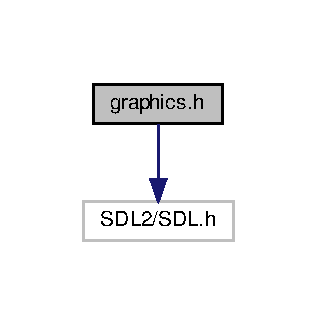
\includegraphics[width=152pt]{graphics_8h__incl}
\end{center}
\end{figure}
This graph shows which files directly or indirectly include this file\+:\nopagebreak
\begin{figure}[H]
\begin{center}
\leavevmode
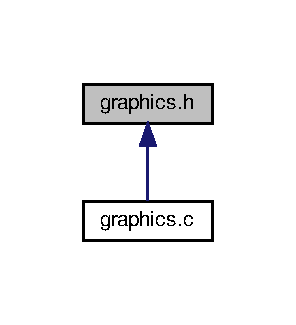
\includegraphics[width=142pt]{graphics_8h__dep__incl}
\end{center}
\end{figure}
\subsection*{Macros}
\begin{DoxyCompactItemize}
\item 
\mbox{\Hypertarget{graphics_8h_a28a1ed26c61aa87880397b3e247b03b7}\label{graphics_8h_a28a1ed26c61aa87880397b3e247b03b7}} 
\#define \hyperlink{graphics_8h_a28a1ed26c61aa87880397b3e247b03b7}{G\+R\+A\+P\+H\+I\+C\+S\+\_\+\+V\+E\+R\+S\+I\+ON}~\char`\"{}0.\+1.\+0\char`\"{}
\begin{DoxyCompactList}\small\item\em include guard \end{DoxyCompactList}\end{DoxyCompactItemize}
\subsection*{Functions}
\begin{DoxyCompactItemize}
\item 
struct \hyperlink{structgraphics}{graphics} $\ast$ \hyperlink{graphics_8h_a543e265f9ff924a1def601674c56b3a2}{Graphics\+Init} (char $\ast$title, int width, int height, int scale)
\begin{DoxyCompactList}\small\item\em Creates and initializes a new graphics object isntance. \end{DoxyCompactList}\item 
void \hyperlink{graphics_8h_a60bfad8b4f1ee06733460378fa8e56e0}{Graphics\+Deinit} (struct \hyperlink{structgraphics}{graphics} $\ast$\hyperlink{structgraphics}{graphics})
\begin{DoxyCompactList}\small\item\em De-\/initializes and frees memory for the given graphics object. \end{DoxyCompactList}\item 
void \hyperlink{graphics_8h_acc8d5ed3b6d471a3df71f6c080f57194}{Graphics\+Begin} (struct \hyperlink{structgraphics}{graphics} $\ast$\hyperlink{structgraphics}{graphics})
\begin{DoxyCompactList}\small\item\em Initializes the graphics subsystem for drawing routines. \end{DoxyCompactList}\item 
void \hyperlink{graphics_8h_a93d049610e6a7de779502b748fe0a84a}{Graphics\+End} (struct \hyperlink{structgraphics}{graphics} $\ast$\hyperlink{structgraphics}{graphics})
\begin{DoxyCompactList}\small\item\em Prepares the graphics subsystem for presentation, then presents. \end{DoxyCompactList}\item 
void \hyperlink{graphics_8h_ac7cff8334dd93066be5801a7a12b00df}{Graphics\+Clear\+Screen} (struct \hyperlink{structgraphics}{graphics} $\ast$\hyperlink{structgraphics}{graphics}, unsigned int \hyperlink{structcolor}{color})
\begin{DoxyCompactList}\small\item\em Sets all pixels in the screen to the given color. \end{DoxyCompactList}\item 
void \hyperlink{graphics_8h_ab4eed4462ddf5c15ca6ee40500850f5f}{Graphics\+Triangle\+Wireframe} (struct \hyperlink{structgraphics}{graphics} $\ast$\hyperlink{structgraphics}{graphics}, struct \hyperlink{structtriangle}{triangle} \hyperlink{structtriangle}{triangle}, unsigned int \hyperlink{structcolor}{color})
\begin{DoxyCompactList}\small\item\em Draw a triangle with the given set of x and y coordinates. \end{DoxyCompactList}\item 
void \hyperlink{graphics_8h_a0ced2380f07dd02a2251f70480c8a0a9}{Graphics\+Triangle\+Solid} (struct \hyperlink{structgraphics}{graphics} $\ast$\hyperlink{structgraphics}{graphics}, struct \hyperlink{structtriangle}{triangle} \hyperlink{structtriangle}{triangle}, unsigned int \hyperlink{structcolor}{color})
\begin{DoxyCompactList}\small\item\em Draw a triangle with the given set of x and y coordinates. \end{DoxyCompactList}\item 
void \hyperlink{graphics_8h_a50ea5ae7900c76984aa7beabaa79532b}{Graphics\+Triangle\+Textured} (struct \hyperlink{structgraphics}{graphics} $\ast$\hyperlink{structgraphics}{graphics}, struct \hyperlink{structtriangle}{triangle} tri, struct \hyperlink{structtexture}{texture} $\ast$\hyperlink{structtexture}{texture})
\begin{DoxyCompactList}\small\item\em Draw a textured triangle with the given set of x and y coordinates. \end{DoxyCompactList}\end{DoxyCompactItemize}


\subsection{Detailed Description}
Drawing interface to the operating system. 

\subsection{Function Documentation}
\mbox{\Hypertarget{graphics_8h_acc8d5ed3b6d471a3df71f6c080f57194}\label{graphics_8h_acc8d5ed3b6d471a3df71f6c080f57194}} 
\index{graphics.\+h@{graphics.\+h}!Graphics\+Begin@{Graphics\+Begin}}
\index{Graphics\+Begin@{Graphics\+Begin}!graphics.\+h@{graphics.\+h}}
\subsubsection{\texorpdfstring{Graphics\+Begin()}{GraphicsBegin()}}
{\footnotesize\ttfamily void Graphics\+Begin (\begin{DoxyParamCaption}\item[{struct \hyperlink{structgraphics}{graphics} $\ast$}]{graphics }\end{DoxyParamCaption})}



Initializes the graphics subsystem for drawing routines. 

Internally locks streaming texture for direct manipulation.


\begin{DoxyParams}[1]{Parameters}
\mbox{\tt in,out}  & {\em graphics} & Graphics state to be manipulated \\
\hline
\end{DoxyParams}
\mbox{\Hypertarget{graphics_8h_ac7cff8334dd93066be5801a7a12b00df}\label{graphics_8h_ac7cff8334dd93066be5801a7a12b00df}} 
\index{graphics.\+h@{graphics.\+h}!Graphics\+Clear\+Screen@{Graphics\+Clear\+Screen}}
\index{Graphics\+Clear\+Screen@{Graphics\+Clear\+Screen}!graphics.\+h@{graphics.\+h}}
\subsubsection{\texorpdfstring{Graphics\+Clear\+Screen()}{GraphicsClearScreen()}}
{\footnotesize\ttfamily void Graphics\+Clear\+Screen (\begin{DoxyParamCaption}\item[{struct \hyperlink{structgraphics}{graphics} $\ast$}]{graphics,  }\item[{unsigned int}]{color }\end{DoxyParamCaption})}



Sets all pixels in the screen to the given color. 


\begin{DoxyParams}[1]{Parameters}
\mbox{\tt in,out}  & {\em graphics} & Graphics state to be manipulated \\
\hline
\mbox{\tt in}  & {\em color} & 32-\/bit color with 8-\/bits per component\+: (R,G,B,A) \\
\hline
\end{DoxyParams}
\mbox{\Hypertarget{graphics_8h_a60bfad8b4f1ee06733460378fa8e56e0}\label{graphics_8h_a60bfad8b4f1ee06733460378fa8e56e0}} 
\index{graphics.\+h@{graphics.\+h}!Graphics\+Deinit@{Graphics\+Deinit}}
\index{Graphics\+Deinit@{Graphics\+Deinit}!graphics.\+h@{graphics.\+h}}
\subsubsection{\texorpdfstring{Graphics\+Deinit()}{GraphicsDeinit()}}
{\footnotesize\ttfamily void Graphics\+Deinit (\begin{DoxyParamCaption}\item[{struct \hyperlink{structgraphics}{graphics} $\ast$}]{graphics }\end{DoxyParamCaption})}



De-\/initializes and frees memory for the given graphics object. 


\begin{DoxyParams}[1]{Parameters}
\mbox{\tt in,out}  & {\em graphics} & The initialized opcode object to be cleaned and reclaimed \\
\hline
\end{DoxyParams}
\mbox{\Hypertarget{graphics_8h_a93d049610e6a7de779502b748fe0a84a}\label{graphics_8h_a93d049610e6a7de779502b748fe0a84a}} 
\index{graphics.\+h@{graphics.\+h}!Graphics\+End@{Graphics\+End}}
\index{Graphics\+End@{Graphics\+End}!graphics.\+h@{graphics.\+h}}
\subsubsection{\texorpdfstring{Graphics\+End()}{GraphicsEnd()}}
{\footnotesize\ttfamily void Graphics\+End (\begin{DoxyParamCaption}\item[{struct \hyperlink{structgraphics}{graphics} $\ast$}]{graphics }\end{DoxyParamCaption})}



Prepares the graphics subsystem for presentation, then presents. 

Internally unlocks streaming texture then calls presentation routines.


\begin{DoxyParams}[1]{Parameters}
\mbox{\tt in,out}  & {\em graphics} & Graphics state to be manipulated. \\
\hline
\end{DoxyParams}
\mbox{\Hypertarget{graphics_8h_a543e265f9ff924a1def601674c56b3a2}\label{graphics_8h_a543e265f9ff924a1def601674c56b3a2}} 
\index{graphics.\+h@{graphics.\+h}!Graphics\+Init@{Graphics\+Init}}
\index{Graphics\+Init@{Graphics\+Init}!graphics.\+h@{graphics.\+h}}
\subsubsection{\texorpdfstring{Graphics\+Init()}{GraphicsInit()}}
{\footnotesize\ttfamily struct \hyperlink{structgraphics}{graphics}$\ast$ Graphics\+Init (\begin{DoxyParamCaption}\item[{char $\ast$}]{title,  }\item[{int}]{width,  }\item[{int}]{height,  }\item[{int}]{scale }\end{DoxyParamCaption})}



Creates and initializes a new graphics object isntance. 

Scale can be specified as a non-\/negative number. This value is used to multiply both the width and the height and the pixel size of any drawing operations.

For example, specifying a scale of 2 would multiply the width by 2, the height by 2, and every pixel would be 2x2; so the total scale factor ends up being scale$^\wedge$2


\begin{DoxyParams}[1]{Parameters}
\mbox{\tt in}  & {\em title} & The title displayed in the window titlebar \\
\hline
\mbox{\tt in}  & {\em width} & Width of the display area of the window, in pixels \\
\hline
\mbox{\tt in}  & {\em height} & Height of the display are of the window, in pixels \\
\hline
\mbox{\tt in}  & {\em scale} & Size and rendering scale, natural number multiple \\
\hline
\end{DoxyParams}
\begin{DoxyReturn}{Returns}
The initialized graphics object 
\end{DoxyReturn}
\mbox{\Hypertarget{graphics_8h_a0ced2380f07dd02a2251f70480c8a0a9}\label{graphics_8h_a0ced2380f07dd02a2251f70480c8a0a9}} 
\index{graphics.\+h@{graphics.\+h}!Graphics\+Triangle\+Solid@{Graphics\+Triangle\+Solid}}
\index{Graphics\+Triangle\+Solid@{Graphics\+Triangle\+Solid}!graphics.\+h@{graphics.\+h}}
\subsubsection{\texorpdfstring{Graphics\+Triangle\+Solid()}{GraphicsTriangleSolid()}}
{\footnotesize\ttfamily void Graphics\+Triangle\+Solid (\begin{DoxyParamCaption}\item[{struct \hyperlink{structgraphics}{graphics} $\ast$}]{graphics,  }\item[{struct \hyperlink{structtriangle}{triangle}}]{triangle,  }\item[{unsigned int}]{color }\end{DoxyParamCaption})}



Draw a triangle with the given set of x and y coordinates. 

Fills the specified polygon with the given color.


\begin{DoxyParams}[1]{Parameters}
\mbox{\tt in,out}  & {\em graphics} & Graphics state to be changed \\
\hline
\mbox{\tt in}  & {\em triangle} & The triangle to draw \\
\hline
\mbox{\tt in}  & {\em color} & What color the solid triangle should be rendered with\\
\hline
\end{DoxyParams}
\begin{DoxySeeAlso}{See also}
Source\+: \href{http://www.sunshine2k.de/coding/java/TriangleRasterization/TriangleRasterization.html}{\tt http\+://www.\+sunshine2k.\+de/coding/java/\+Triangle\+Rasterization/\+Triangle\+Rasterization.\+html} 
\end{DoxySeeAlso}
\mbox{\Hypertarget{graphics_8h_a50ea5ae7900c76984aa7beabaa79532b}\label{graphics_8h_a50ea5ae7900c76984aa7beabaa79532b}} 
\index{graphics.\+h@{graphics.\+h}!Graphics\+Triangle\+Textured@{Graphics\+Triangle\+Textured}}
\index{Graphics\+Triangle\+Textured@{Graphics\+Triangle\+Textured}!graphics.\+h@{graphics.\+h}}
\subsubsection{\texorpdfstring{Graphics\+Triangle\+Textured()}{GraphicsTriangleTextured()}}
{\footnotesize\ttfamily void Graphics\+Triangle\+Textured (\begin{DoxyParamCaption}\item[{struct \hyperlink{structgraphics}{graphics} $\ast$}]{graphics,  }\item[{struct \hyperlink{structtriangle}{triangle}}]{tri,  }\item[{struct \hyperlink{structtexture}{texture} $\ast$}]{texture }\end{DoxyParamCaption})}



Draw a textured triangle with the given set of x and y coordinates. 

Fills the specified polygon with the given texture.


\begin{DoxyParams}[1]{Parameters}
\mbox{\tt in,out}  & {\em graphics} & Graphics state to be changed \\
\hline
\mbox{\tt in}  & {\em tri} & The triangle to draw \\
\hline
\mbox{\tt in}  & {\em texture} & What texture to sample while drawing the solid triangle\\
\hline
\end{DoxyParams}
\begin{DoxySeeAlso}{See also}
Source\+: \href{https://github.com/OneLoneCoder/videos/blob/master/OneLoneCoder_olcEngine3D_Part4.cpp}{\tt https\+://github.\+com/\+One\+Lone\+Coder/videos/blob/master/\+One\+Lone\+Coder\+\_\+olc\+Engine3\+D\+\_\+\+Part4.\+cpp} 
\end{DoxySeeAlso}
\mbox{\Hypertarget{graphics_8h_ab4eed4462ddf5c15ca6ee40500850f5f}\label{graphics_8h_ab4eed4462ddf5c15ca6ee40500850f5f}} 
\index{graphics.\+h@{graphics.\+h}!Graphics\+Triangle\+Wireframe@{Graphics\+Triangle\+Wireframe}}
\index{Graphics\+Triangle\+Wireframe@{Graphics\+Triangle\+Wireframe}!graphics.\+h@{graphics.\+h}}
\subsubsection{\texorpdfstring{Graphics\+Triangle\+Wireframe()}{GraphicsTriangleWireframe()}}
{\footnotesize\ttfamily void Graphics\+Triangle\+Wireframe (\begin{DoxyParamCaption}\item[{struct \hyperlink{structgraphics}{graphics} $\ast$}]{graphics,  }\item[{struct \hyperlink{structtriangle}{triangle}}]{triangle,  }\item[{unsigned int}]{color }\end{DoxyParamCaption})}



Draw a triangle with the given set of x and y coordinates. 

Only draws the lines, doesn\textquotesingle{}t fill the polygon.


\begin{DoxyParams}[1]{Parameters}
\mbox{\tt in,out}  & {\em graphics} & Graphics state to be changed \\
\hline
\mbox{\tt in}  & {\em triangle} & The triangle to draw \\
\hline
\mbox{\tt in}  & {\em color} & What color the wireframe should be rendered with \\
\hline
\end{DoxyParams}

\hypertarget{input_8c}{}\section{input.\+c File Reference}
\label{input_8c}\index{input.\+c@{input.\+c}}
{\ttfamily \#include \char`\"{}S\+D\+L2/\+S\+D\+L.\+h\char`\"{}}\newline
{\ttfamily \#include \char`\"{}math.\+h\char`\"{}}\newline
Include dependency graph for input.\+c\+:\nopagebreak
\begin{figure}[H]
\begin{center}
\leavevmode
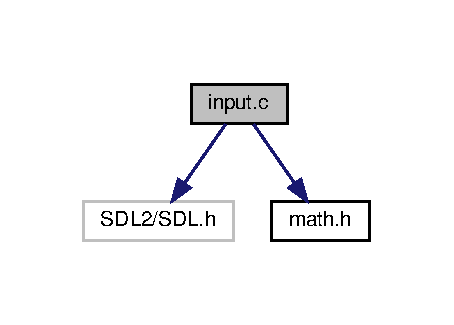
\includegraphics[width=218pt]{input_8c__incl}
\end{center}
\end{figure}
\subsection*{Classes}
\begin{DoxyCompactItemize}
\item 
struct \hyperlink{structinput}{input}
\begin{DoxyCompactList}\small\item\em Keypress state. Unexported. \end{DoxyCompactList}\end{DoxyCompactItemize}
\subsection*{Functions}
\begin{DoxyCompactItemize}
\item 
struct \hyperlink{structinput}{input} $\ast$ \hyperlink{input_8c_a1d6bc79955841788279b2eb5cf12d390}{Input\+Init} ()
\begin{DoxyCompactList}\small\item\em Creates and initializes a new input object. \end{DoxyCompactList}\item 
void \hyperlink{input_8c_a68054d62d814fb092e0927f163d0e8ad}{Input\+Deinit} (struct \hyperlink{structinput}{input} $\ast$i)
\begin{DoxyCompactList}\small\item\em De-\/initializes and frees memory for the given input object. \end{DoxyCompactList}\item 
\mbox{\Hypertarget{input_8c_a5f5f8ed38e1c000d6441daf26922e043}\label{input_8c_a5f5f8ed38e1c000d6441daf26922e043}} 
int {\bfseries Input\+Is\+Quit\+Pressed} (struct \hyperlink{structinput}{input} $\ast$i, S\+D\+L\+\_\+\+Event $\ast$event)
\item 
void \hyperlink{input_8c_a9d53e96b684d7f742ce3864ca5b0e656}{Input\+Process} (struct \hyperlink{structinput}{input} $\ast$i)
\begin{DoxyCompactList}\small\item\em Handle input. \end{DoxyCompactList}\end{DoxyCompactItemize}
\subsection*{Variables}
\begin{DoxyCompactItemize}
\item 
\mbox{\Hypertarget{input_8c_a3424564b22c110ebf7cbfc61eae2709d}\label{input_8c_a3424564b22c110ebf7cbfc61eae2709d}} 
struct \hyperlink{structvec3}{vec3} {\bfseries camera}
\item 
\mbox{\Hypertarget{input_8c_af00c9a33a2edf335eb87b8d56735ffe8}\label{input_8c_af00c9a33a2edf335eb87b8d56735ffe8}} 
struct \hyperlink{structvec3}{vec3} {\bfseries look\+Dir}
\item 
\mbox{\Hypertarget{input_8c_a3606c0811ea504b10ef1e666f2de161c}\label{input_8c_a3606c0811ea504b10ef1e666f2de161c}} 
struct \hyperlink{structvec3}{vec3} {\bfseries up}
\item 
\mbox{\Hypertarget{input_8c_a7efc219781df4a1e281cb5d348b7fbf9}\label{input_8c_a7efc219781df4a1e281cb5d348b7fbf9}} 
float {\bfseries yaw}
\item 
\mbox{\Hypertarget{input_8c_a57f63506d2191a58a41afec3c3060221}\label{input_8c_a57f63506d2191a58a41afec3c3060221}} 
double {\bfseries elapsed\+Time}
\end{DoxyCompactItemize}


\subsection{Function Documentation}
\mbox{\Hypertarget{input_8c_a68054d62d814fb092e0927f163d0e8ad}\label{input_8c_a68054d62d814fb092e0927f163d0e8ad}} 
\index{input.\+c@{input.\+c}!Input\+Deinit@{Input\+Deinit}}
\index{Input\+Deinit@{Input\+Deinit}!input.\+c@{input.\+c}}
\subsubsection{\texorpdfstring{Input\+Deinit()}{InputDeinit()}}
{\footnotesize\ttfamily void Input\+Deinit (\begin{DoxyParamCaption}\item[{struct \hyperlink{structinput}{input} $\ast$}]{input }\end{DoxyParamCaption})}



De-\/initializes and frees memory for the given input object. 


\begin{DoxyParams}[1]{Parameters}
\mbox{\tt in,out}  & {\em input} & The initialized input object to be cleaned and reclaimed \\
\hline
\end{DoxyParams}
\mbox{\Hypertarget{input_8c_a1d6bc79955841788279b2eb5cf12d390}\label{input_8c_a1d6bc79955841788279b2eb5cf12d390}} 
\index{input.\+c@{input.\+c}!Input\+Init@{Input\+Init}}
\index{Input\+Init@{Input\+Init}!input.\+c@{input.\+c}}
\subsubsection{\texorpdfstring{Input\+Init()}{InputInit()}}
{\footnotesize\ttfamily struct \hyperlink{structinput}{input}$\ast$ Input\+Init (\begin{DoxyParamCaption}{ }\end{DoxyParamCaption})}



Creates and initializes a new input object. 

\begin{DoxyReturn}{Returns}
The initialized input object 
\end{DoxyReturn}
\mbox{\Hypertarget{input_8c_a9d53e96b684d7f742ce3864ca5b0e656}\label{input_8c_a9d53e96b684d7f742ce3864ca5b0e656}} 
\index{input.\+c@{input.\+c}!Input\+Process@{Input\+Process}}
\index{Input\+Process@{Input\+Process}!input.\+c@{input.\+c}}
\subsubsection{\texorpdfstring{Input\+Process()}{InputProcess()}}
{\footnotesize\ttfamily void Input\+Process (\begin{DoxyParamCaption}\item[{struct \hyperlink{structinput}{input} $\ast$}]{input }\end{DoxyParamCaption})}



Handle input. 


\begin{DoxyParams}[1]{Parameters}
\mbox{\tt in,out}  & {\em input} & Input state to be updated \\
\hline
\mbox{\tt in}  & {\em event} & S\+DL event to process \\
\hline
\end{DoxyParams}

\hypertarget{input_8h}{}\section{input.\+h File Reference}
\label{input_8h}\index{input.\+h@{input.\+h}}
{\ttfamily \#include \char`\"{}S\+D\+L.\+h\char`\"{}}\newline
Include dependency graph for input.\+h\+:\nopagebreak
\begin{figure}[H]
\begin{center}
\leavevmode
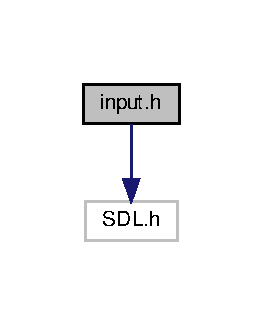
\includegraphics[width=126pt]{input_8h__incl}
\end{center}
\end{figure}
\subsection*{Macros}
\begin{DoxyCompactItemize}
\item 
\mbox{\Hypertarget{input_8h_abca4f285fc582fc00029c078fdee9e82}\label{input_8h_abca4f285fc582fc00029c078fdee9e82}} 
\#define {\bfseries I\+N\+P\+U\+T\+\_\+\+V\+E\+R\+S\+I\+ON}~\char`\"{}0.\+1.\+0\char`\"{}
\end{DoxyCompactItemize}
\subsection*{Functions}
\begin{DoxyCompactItemize}
\item 
struct \hyperlink{structinput}{input} $\ast$ \hyperlink{input_8h_a1d6bc79955841788279b2eb5cf12d390}{Input\+Init} ()
\begin{DoxyCompactList}\small\item\em Creates and initializes a new input object. \end{DoxyCompactList}\item 
void \hyperlink{input_8h_a6767724b756cbf018c89f333927b2a60}{Input\+Deinit} (struct \hyperlink{structinput}{input} $\ast$\hyperlink{structinput}{input})
\begin{DoxyCompactList}\small\item\em De-\/initializes and frees memory for the given input object. \end{DoxyCompactList}\item 
\mbox{\Hypertarget{input_8h_a648e479124b096d398b8ff155a4c8ec2}\label{input_8h_a648e479124b096d398b8ff155a4c8ec2}} 
int {\bfseries Input\+Is\+Quit\+Pressed} (struct \hyperlink{structinput}{input} $\ast$\hyperlink{structinput}{input}, S\+D\+L\+\_\+\+Event $\ast$event)
\item 
void \hyperlink{input_8h_ac1731aedf34349137cd066e474a8b0d2}{Input\+Process} (struct \hyperlink{structinput}{input} $\ast$\hyperlink{structinput}{input})
\begin{DoxyCompactList}\small\item\em Handle input. \end{DoxyCompactList}\end{DoxyCompactItemize}


\subsection{Detailed Description}
This package provides a small input abstraction layer to separate input processing from system emulation. Input operates in the same thread as graphics, at the same frequency (30hz) and calls back into the system emulation thread. 

\subsection{Function Documentation}
\mbox{\Hypertarget{input_8h_a6767724b756cbf018c89f333927b2a60}\label{input_8h_a6767724b756cbf018c89f333927b2a60}} 
\index{input.\+h@{input.\+h}!Input\+Deinit@{Input\+Deinit}}
\index{Input\+Deinit@{Input\+Deinit}!input.\+h@{input.\+h}}
\subsubsection{\texorpdfstring{Input\+Deinit()}{InputDeinit()}}
{\footnotesize\ttfamily void Input\+Deinit (\begin{DoxyParamCaption}\item[{struct \hyperlink{structinput}{input} $\ast$}]{input }\end{DoxyParamCaption})}



De-\/initializes and frees memory for the given input object. 


\begin{DoxyParams}[1]{Parameters}
\mbox{\tt in,out}  & {\em input} & The initialized input object to be cleaned and reclaimed \\
\hline
\end{DoxyParams}
\mbox{\Hypertarget{input_8h_a1d6bc79955841788279b2eb5cf12d390}\label{input_8h_a1d6bc79955841788279b2eb5cf12d390}} 
\index{input.\+h@{input.\+h}!Input\+Init@{Input\+Init}}
\index{Input\+Init@{Input\+Init}!input.\+h@{input.\+h}}
\subsubsection{\texorpdfstring{Input\+Init()}{InputInit()}}
{\footnotesize\ttfamily struct \hyperlink{structinput}{input}$\ast$ Input\+Init (\begin{DoxyParamCaption}{ }\end{DoxyParamCaption})}



Creates and initializes a new input object. 

\begin{DoxyReturn}{Returns}
The initialized input object 
\end{DoxyReturn}
\mbox{\Hypertarget{input_8h_ac1731aedf34349137cd066e474a8b0d2}\label{input_8h_ac1731aedf34349137cd066e474a8b0d2}} 
\index{input.\+h@{input.\+h}!Input\+Process@{Input\+Process}}
\index{Input\+Process@{Input\+Process}!input.\+h@{input.\+h}}
\subsubsection{\texorpdfstring{Input\+Process()}{InputProcess()}}
{\footnotesize\ttfamily void Input\+Process (\begin{DoxyParamCaption}\item[{struct \hyperlink{structinput}{input} $\ast$}]{input }\end{DoxyParamCaption})}



Handle input. 


\begin{DoxyParams}[1]{Parameters}
\mbox{\tt in,out}  & {\em input} & Input state to be updated \\
\hline
\mbox{\tt in}  & {\em event} & S\+DL event to process \\
\hline
\end{DoxyParams}

\hypertarget{math_8c}{}\section{math.\+c File Reference}
\label{math_8c}\index{math.\+c@{math.\+c}}
{\ttfamily \#include $<$stdlib.\+h$>$}\newline
{\ttfamily \#include $<$string.\+h$>$}\newline
{\ttfamily \#include $<$stdio.\+h$>$}\newline
{\ttfamily \#include $<$math.\+h$>$}\newline
{\ttfamily \#include \char`\"{}color.\+h\char`\"{}}\newline
Include dependency graph for math.\+c\+:\nopagebreak
\begin{figure}[H]
\begin{center}
\leavevmode
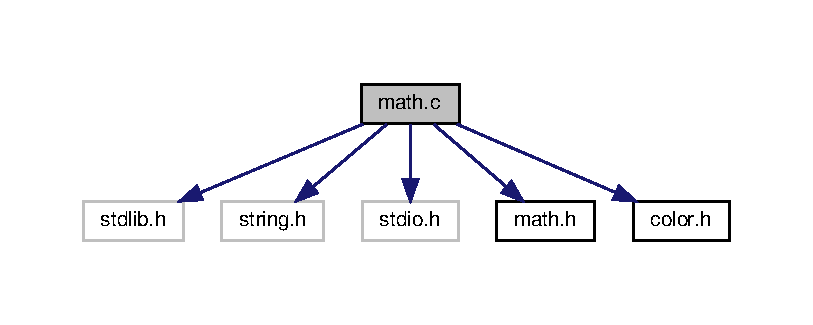
\includegraphics[width=350pt]{math_8c__incl}
\end{center}
\end{figure}
\subsection*{Functions}
\begin{DoxyCompactItemize}
\item 
\mbox{\Hypertarget{math_8c_a8c9261cf5fecb28a6b1a91f8539fff5f}\label{math_8c_a8c9261cf5fecb28a6b1a91f8539fff5f}} 
struct \hyperlink{structvec3}{vec3} {\bfseries Vec3\+Init} (float x, float y, float z)
\item 
\mbox{\Hypertarget{math_8c_af84878c945636c9983379337bfddb2f6}\label{math_8c_af84878c945636c9983379337bfddb2f6}} 
void {\bfseries Vec3\+Debug} (struct \hyperlink{structvec3}{vec3} v, char $\ast$name)
\item 
\mbox{\Hypertarget{math_8c_adcc7a783bbf899d67a1c562ab853317e}\label{math_8c_adcc7a783bbf899d67a1c562ab853317e}} 
void {\bfseries Triangle\+Debug} (struct \hyperlink{structtriangle}{triangle} t, char $\ast$name)
\item 
\mbox{\Hypertarget{math_8c_a45f881ac817d47d7c3e6847bdda33dac}\label{math_8c_a45f881ac817d47d7c3e6847bdda33dac}} 
float {\bfseries Vec3\+Dot\+Product} (struct \hyperlink{structvec3}{vec3} left, struct \hyperlink{structvec3}{vec3} right)
\item 
\mbox{\Hypertarget{math_8c_a69e10952072b5703de2b90626b946ce8}\label{math_8c_a69e10952072b5703de2b90626b946ce8}} 
struct \hyperlink{structvec3}{vec3} {\bfseries Vec3\+Cross\+Product} (struct \hyperlink{structvec3}{vec3} left, struct \hyperlink{structvec3}{vec3} right)
\item 
\mbox{\Hypertarget{math_8c_addd3f3db8991b69c527cec7dde2e5f1b}\label{math_8c_addd3f3db8991b69c527cec7dde2e5f1b}} 
struct \hyperlink{structvec3}{vec3} {\bfseries Vec3\+Normalize} (struct \hyperlink{structvec3}{vec3} \hyperlink{structvec3}{vec3})
\item 
\mbox{\Hypertarget{math_8c_a28bc0a705a413c38975439be9103a033}\label{math_8c_a28bc0a705a413c38975439be9103a033}} 
struct \hyperlink{structvec3}{vec3} {\bfseries Vec3\+Add} (struct \hyperlink{structvec3}{vec3} left, struct \hyperlink{structvec3}{vec3} right)
\item 
\mbox{\Hypertarget{math_8c_ac45af7fec431d52532be07da335b3adc}\label{math_8c_ac45af7fec431d52532be07da335b3adc}} 
struct \hyperlink{structvec3}{vec3} {\bfseries Vec3\+Subtract} (struct \hyperlink{structvec3}{vec3} minuend, struct \hyperlink{structvec3}{vec3} subtrahend)
\item 
\mbox{\Hypertarget{math_8c_a54a5fb2c28d7239e5f9587be2c1a33e7}\label{math_8c_a54a5fb2c28d7239e5f9587be2c1a33e7}} 
struct \hyperlink{structvec3}{vec3} {\bfseries Vec3\+Multiply} (struct \hyperlink{structvec3}{vec3} \hyperlink{structvec3}{vec3}, float f)
\item 
\mbox{\Hypertarget{math_8c_a2d73aa92e59d061d47fec9f5fdfdca98}\label{math_8c_a2d73aa92e59d061d47fec9f5fdfdca98}} 
struct \hyperlink{structvec3}{vec3} {\bfseries Vec3\+Divide} (struct \hyperlink{structvec3}{vec3} \hyperlink{structvec3}{vec3}, float f)
\item 
struct \hyperlink{structvec3}{vec3} \hyperlink{math_8c_abe3a401d048f138be1b2667dba51b0e1}{Vec3\+Intersect\+Plane} (struct \hyperlink{structvec3}{vec3} point, struct \hyperlink{structvec3}{vec3} normal, struct \hyperlink{structvec3}{vec3} line\+Start, struct \hyperlink{structvec3}{vec3} line\+End, float $\ast$t)
\begin{DoxyCompactList}\small\item\em Return the 3d point where a line intersects a plane. \end{DoxyCompactList}\item 
\mbox{\Hypertarget{math_8c_ac8ca162e93ba251e02dc91ba8d3bedde}\label{math_8c_ac8ca162e93ba251e02dc91ba8d3bedde}} 
float \hyperlink{math_8c_ac8ca162e93ba251e02dc91ba8d3bedde}{Shortest\+Dist\+To\+Plane} (struct \hyperlink{structvec3}{vec3} point, struct \hyperlink{structvec3}{vec3} plane\+Point, struct \hyperlink{structvec3}{vec3} plane\+Normal)
\begin{DoxyCompactList}\small\item\em Return shortest distance from point to plan given a normalized normal. \end{DoxyCompactList}\item 
\mbox{\Hypertarget{math_8c_a09061f35aa26ac2ea241c53a89982dbe}\label{math_8c_a09061f35aa26ac2ea241c53a89982dbe}} 
struct \hyperlink{structtriangle}{triangle} \hyperlink{math_8c_a09061f35aa26ac2ea241c53a89982dbe}{Triangle\+Init} (float x1, float y1, float z1, float u1, float v1, float x2, float y2, float z2, float u2, float v2, float x3, float y3, float z3, float u3, float v3)
\begin{DoxyCompactList}\small\item\em Create a new triangle with the given params. \end{DoxyCompactList}\item 
int \hyperlink{math_8c_ad5746897eb2f3a6dcf661385638a3e4d}{Triangle\+Clip\+Against\+Plane} (struct \hyperlink{structvec3}{vec3} plane, struct \hyperlink{structvec3}{vec3} normal, struct \hyperlink{structtriangle}{triangle} in, struct \hyperlink{structtriangle}{triangle} $\ast$out1, struct \hyperlink{structtriangle}{triangle} $\ast$out2)
\begin{DoxyCompactList}\small\item\em Clip a triangle against a plane. \end{DoxyCompactList}\item 
\mbox{\Hypertarget{math_8c_a9c277ea118c7764f5373a812c1793912}\label{math_8c_a9c277ea118c7764f5373a812c1793912}} 
struct \hyperlink{structmesh}{mesh} $\ast$ {\bfseries Mesh\+Init} (int num\+Tris)
\item 
\mbox{\Hypertarget{math_8c_acc332ef7c45f7d2b41eea974cd4586e9}\label{math_8c_acc332ef7c45f7d2b41eea974cd4586e9}} 
struct \hyperlink{structmesh}{mesh} $\ast$ {\bfseries Mesh\+Init\+From\+Obj} (char $\ast$obj\+File)
\item 
\mbox{\Hypertarget{math_8c_a42944cfe95cfee1a57bceb58c46e5bca}\label{math_8c_a42944cfe95cfee1a57bceb58c46e5bca}} 
void {\bfseries Mesh\+Deinit} (struct \hyperlink{structmesh}{mesh} $\ast$\hyperlink{structmesh}{mesh})
\item 
\mbox{\Hypertarget{math_8c_aa7d3b02d31d5ab0cf16b0127a2a09caa}\label{math_8c_aa7d3b02d31d5ab0cf16b0127a2a09caa}} 
struct \hyperlink{structvec3}{vec3} {\bfseries Mat4x4\+Multiply\+Vec3} (struct \hyperlink{structmat4x4}{mat4x4} mat, struct \hyperlink{structvec3}{vec3} vec)
\item 
\mbox{\Hypertarget{math_8c_aa92ee0c4bea76acbfb1749fce35a4382}\label{math_8c_aa92ee0c4bea76acbfb1749fce35a4382}} 
struct \hyperlink{structmat4x4}{mat4x4} {\bfseries Mat4x4\+Identity} ()
\item 
\mbox{\Hypertarget{math_8c_a32c492937f7697acd790880f481a9eb1}\label{math_8c_a32c492937f7697acd790880f481a9eb1}} 
struct \hyperlink{structmat4x4}{mat4x4} {\bfseries Mat4x4\+RotateX} (float rad)
\item 
\mbox{\Hypertarget{math_8c_af839e81a964a7405f50d2f6427cefedd}\label{math_8c_af839e81a964a7405f50d2f6427cefedd}} 
struct \hyperlink{structmat4x4}{mat4x4} {\bfseries Mat4x4\+RotateY} (float rad)
\item 
\mbox{\Hypertarget{math_8c_a8ebbf465e313b1a5513e0ecda5b73531}\label{math_8c_a8ebbf465e313b1a5513e0ecda5b73531}} 
struct \hyperlink{structmat4x4}{mat4x4} {\bfseries Mat4x4\+RotateZ} (float rad)
\item 
\mbox{\Hypertarget{math_8c_a8999d44c678e4c685203e8c096af5ea4}\label{math_8c_a8999d44c678e4c685203e8c096af5ea4}} 
struct \hyperlink{structmat4x4}{mat4x4} {\bfseries Mat4x4\+Translate} (float x, float y, float z)
\item 
\mbox{\Hypertarget{math_8c_a24a5562b24e935847209d413d6bd6e1b}\label{math_8c_a24a5562b24e935847209d413d6bd6e1b}} 
struct \hyperlink{structmat4x4}{mat4x4} {\bfseries Mat4x4\+Project} (float fov\+Degrees, float aspect, float near, float far)
\item 
\mbox{\Hypertarget{math_8c_ae691972849ade4a1f328ef9be0b1e442}\label{math_8c_ae691972849ade4a1f328ef9be0b1e442}} 
struct \hyperlink{structmat4x4}{mat4x4} {\bfseries Mat4x4\+Multiply} (struct \hyperlink{structmat4x4}{mat4x4} left, struct \hyperlink{structmat4x4}{mat4x4} right)
\item 
\mbox{\Hypertarget{math_8c_a7548490f5b0f671ed4d451e70cf09180}\label{math_8c_a7548490f5b0f671ed4d451e70cf09180}} 
struct \hyperlink{structmat4x4}{mat4x4} \hyperlink{math_8c_a7548490f5b0f671ed4d451e70cf09180}{Mat4x4\+Invert\+Fast} (struct \hyperlink{structmat4x4}{mat4x4} matrix)
\begin{DoxyCompactList}\small\item\em Fast matrix inverse. Doesn\textquotesingle{}t work if matrix does scaling. \end{DoxyCompactList}\item 
\mbox{\Hypertarget{math_8c_ac0e023300a38e34bea1666e3f83d296d}\label{math_8c_ac0e023300a38e34bea1666e3f83d296d}} 
struct \hyperlink{structmat4x4}{mat4x4} {\bfseries Mat4x4\+Point\+At} (struct \hyperlink{structvec3}{vec3} pos, struct \hyperlink{structvec3}{vec3} target, struct \hyperlink{structvec3}{vec3} up)
\item 
\mbox{\Hypertarget{math_8c_a34ca5ff0093e0b5c52af53e072aeb798}\label{math_8c_a34ca5ff0093e0b5c52af53e072aeb798}} 
void {\bfseries Mat4x4\+Debug} (struct \hyperlink{structmat4x4}{mat4x4} mat, char $\ast$name)
\end{DoxyCompactItemize}


\subsection{Function Documentation}
\mbox{\Hypertarget{math_8c_ad5746897eb2f3a6dcf661385638a3e4d}\label{math_8c_ad5746897eb2f3a6dcf661385638a3e4d}} 
\index{math.\+c@{math.\+c}!Triangle\+Clip\+Against\+Plane@{Triangle\+Clip\+Against\+Plane}}
\index{Triangle\+Clip\+Against\+Plane@{Triangle\+Clip\+Against\+Plane}!math.\+c@{math.\+c}}
\subsubsection{\texorpdfstring{Triangle\+Clip\+Against\+Plane()}{TriangleClipAgainstPlane()}}
{\footnotesize\ttfamily int Triangle\+Clip\+Against\+Plane (\begin{DoxyParamCaption}\item[{struct \hyperlink{structvec3}{vec3}}]{plane,  }\item[{struct \hyperlink{structvec3}{vec3}}]{normal,  }\item[{struct \hyperlink{structtriangle}{triangle}}]{in,  }\item[{struct \hyperlink{structtriangle}{triangle} $\ast$}]{out1,  }\item[{struct \hyperlink{structtriangle}{triangle} $\ast$}]{out2 }\end{DoxyParamCaption})}



Clip a triangle against a plane. 

Given a triangle and a plane, if some of the points lie on one side of the plane and some on the other, then split the triangle into 1 or 2 smaller triangles that do not pass through the plane.


\begin{DoxyParams}{Parameters}
{\em plane} & point on the plane to clip against \\
\hline
{\em normal} & normal of the plane to clip against \\
\hline
{\em in} & the triangle to clip \\
\hline
{\em out1} & one of the smaller triangles resulting from the clipping, if necessary \\
\hline
{\em out2} & one of the smaller triangles resulting from the clipping, if necessary \\
\hline
\end{DoxyParams}
\begin{DoxyReturn}{Returns}
0 if all points are outside the plane, 1 if the triangle is not clipped, otherwise the number of smaller triangles resulting from clipping. 
\end{DoxyReturn}
\mbox{\Hypertarget{math_8c_abe3a401d048f138be1b2667dba51b0e1}\label{math_8c_abe3a401d048f138be1b2667dba51b0e1}} 
\index{math.\+c@{math.\+c}!Vec3\+Intersect\+Plane@{Vec3\+Intersect\+Plane}}
\index{Vec3\+Intersect\+Plane@{Vec3\+Intersect\+Plane}!math.\+c@{math.\+c}}
\subsubsection{\texorpdfstring{Vec3\+Intersect\+Plane()}{Vec3IntersectPlane()}}
{\footnotesize\ttfamily struct \hyperlink{structvec3}{vec3} Vec3\+Intersect\+Plane (\begin{DoxyParamCaption}\item[{struct \hyperlink{structvec3}{vec3}}]{plane,  }\item[{struct \hyperlink{structvec3}{vec3}}]{normal,  }\item[{struct \hyperlink{structvec3}{vec3}}]{line\+Start,  }\item[{struct \hyperlink{structvec3}{vec3}}]{line\+End,  }\item[{float $\ast$}]{t }\end{DoxyParamCaption})}



Return the 3d point where a line intersects a plane. 


\begin{DoxyParams}[1]{Parameters}
\mbox{\tt in}  & {\em plane} & 3d point on the plane to intersect against \\
\hline
\mbox{\tt in}  & {\em normal} & normal of the plane to intersect against \\
\hline
\mbox{\tt in}  & {\em line\+Start} & \\
\hline
\mbox{\tt in}  & {\em line\+End} & \\
\hline
\mbox{\tt out}  & {\em t} & where on the line the intersection occurs. \\
\hline
\end{DoxyParams}

\hypertarget{math_8h}{}\section{math.\+h File Reference}
\label{math_8h}\index{math.\+h@{math.\+h}}
This graph shows which files directly or indirectly include this file\+:\nopagebreak
\begin{figure}[H]
\begin{center}
\leavevmode
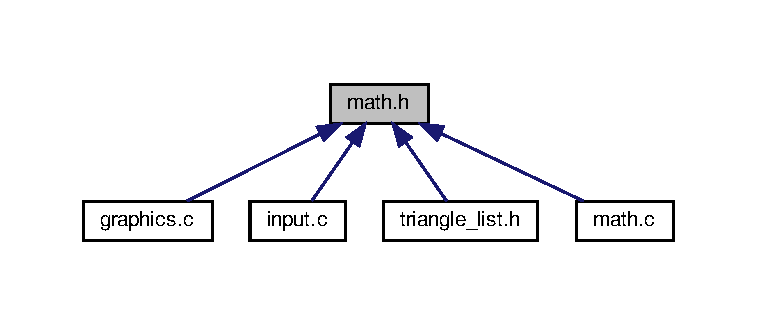
\includegraphics[width=350pt]{math_8h__dep__incl}
\end{center}
\end{figure}
\subsection*{Classes}
\begin{DoxyCompactItemize}
\item 
struct \hyperlink{structvec2}{vec2}
\begin{DoxyCompactList}\small\item\em Homogenous 2D coordinates. \end{DoxyCompactList}\item 
struct \hyperlink{structvec3}{vec3}
\begin{DoxyCompactList}\small\item\em Homogenous 3D coordinates. \end{DoxyCompactList}\item 
struct \hyperlink{structtriangle}{triangle}
\begin{DoxyCompactList}\small\item\em Triangular mesh face. \end{DoxyCompactList}\item 
struct \hyperlink{structmesh}{mesh}
\begin{DoxyCompactList}\small\item\em A collection of triangles representing some kind of 3D model. \end{DoxyCompactList}\item 
struct \hyperlink{structmat4x4}{mat4x4}
\end{DoxyCompactItemize}
\subsection*{Macros}
\begin{DoxyCompactItemize}
\item 
\#define \hyperlink{math_8h_a2171b80d3e540c232ceb5542f172ddb4}{M\+A\+T\+H\+\_\+\+V\+E\+R\+S\+I\+ON}~\char`\"{}0.\+1.\+0\char`\"{}
\begin{DoxyCompactList}\small\item\em A collection of vector and matrix types and associated functions. \end{DoxyCompactList}\end{DoxyCompactItemize}
\subsection*{Functions}
\begin{DoxyCompactItemize}
\item 
\mbox{\Hypertarget{math_8h_a008825dd8d5b07d04ce7441a4342aae0}\label{math_8h_a008825dd8d5b07d04ce7441a4342aae0}} 
void {\bfseries Vec3\+Debug} (struct \hyperlink{structvec3}{vec3} \hyperlink{structvec3}{vec3}, char $\ast$name)
\item 
\mbox{\Hypertarget{math_8h_a8c9261cf5fecb28a6b1a91f8539fff5f}\label{math_8h_a8c9261cf5fecb28a6b1a91f8539fff5f}} 
struct \hyperlink{structvec3}{vec3} {\bfseries Vec3\+Init} (float x, float y, float z)
\item 
\mbox{\Hypertarget{math_8h_a45f881ac817d47d7c3e6847bdda33dac}\label{math_8h_a45f881ac817d47d7c3e6847bdda33dac}} 
float {\bfseries Vec3\+Dot\+Product} (struct \hyperlink{structvec3}{vec3} left, struct \hyperlink{structvec3}{vec3} right)
\item 
\mbox{\Hypertarget{math_8h_a69e10952072b5703de2b90626b946ce8}\label{math_8h_a69e10952072b5703de2b90626b946ce8}} 
struct \hyperlink{structvec3}{vec3} {\bfseries Vec3\+Cross\+Product} (struct \hyperlink{structvec3}{vec3} left, struct \hyperlink{structvec3}{vec3} right)
\item 
\mbox{\Hypertarget{math_8h_addd3f3db8991b69c527cec7dde2e5f1b}\label{math_8h_addd3f3db8991b69c527cec7dde2e5f1b}} 
struct \hyperlink{structvec3}{vec3} {\bfseries Vec3\+Normalize} (struct \hyperlink{structvec3}{vec3} \hyperlink{structvec3}{vec3})
\item 
\mbox{\Hypertarget{math_8h_a28bc0a705a413c38975439be9103a033}\label{math_8h_a28bc0a705a413c38975439be9103a033}} 
struct \hyperlink{structvec3}{vec3} {\bfseries Vec3\+Add} (struct \hyperlink{structvec3}{vec3} left, struct \hyperlink{structvec3}{vec3} right)
\item 
\mbox{\Hypertarget{math_8h_ac45af7fec431d52532be07da335b3adc}\label{math_8h_ac45af7fec431d52532be07da335b3adc}} 
struct \hyperlink{structvec3}{vec3} {\bfseries Vec3\+Subtract} (struct \hyperlink{structvec3}{vec3} minuend, struct \hyperlink{structvec3}{vec3} subtrahend)
\item 
\mbox{\Hypertarget{math_8h_a54a5fb2c28d7239e5f9587be2c1a33e7}\label{math_8h_a54a5fb2c28d7239e5f9587be2c1a33e7}} 
struct \hyperlink{structvec3}{vec3} {\bfseries Vec3\+Multiply} (struct \hyperlink{structvec3}{vec3} \hyperlink{structvec3}{vec3}, float f)
\item 
\mbox{\Hypertarget{math_8h_a2d73aa92e59d061d47fec9f5fdfdca98}\label{math_8h_a2d73aa92e59d061d47fec9f5fdfdca98}} 
struct \hyperlink{structvec3}{vec3} {\bfseries Vec3\+Divide} (struct \hyperlink{structvec3}{vec3} \hyperlink{structvec3}{vec3}, float f)
\item 
struct \hyperlink{structvec3}{vec3} \hyperlink{math_8h_a2cd91f0930e906666c7eff1e6089ee38}{Vec3\+Intersect\+Plane} (struct \hyperlink{structvec3}{vec3} plane, struct \hyperlink{structvec3}{vec3} normal, struct \hyperlink{structvec3}{vec3} line\+Start, struct \hyperlink{structvec3}{vec3} line\+End, float $\ast$t)
\begin{DoxyCompactList}\small\item\em Return the 3d point where a line intersects a plane. \end{DoxyCompactList}\item 
\mbox{\Hypertarget{math_8h_a09061f35aa26ac2ea241c53a89982dbe}\label{math_8h_a09061f35aa26ac2ea241c53a89982dbe}} 
struct \hyperlink{structtriangle}{triangle} \hyperlink{math_8h_a09061f35aa26ac2ea241c53a89982dbe}{Triangle\+Init} (float x1, float y1, float z1, float u1, float v1, float x2, float y2, float z2, float u2, float v2, float x3, float y3, float z3, float u3, float v3)
\begin{DoxyCompactList}\small\item\em Create a new triangle with the given params. \end{DoxyCompactList}\item 
int \hyperlink{math_8h_ad5746897eb2f3a6dcf661385638a3e4d}{Triangle\+Clip\+Against\+Plane} (struct \hyperlink{structvec3}{vec3} plane, struct \hyperlink{structvec3}{vec3} normal, struct \hyperlink{structtriangle}{triangle} in, struct \hyperlink{structtriangle}{triangle} $\ast$out1, struct \hyperlink{structtriangle}{triangle} $\ast$out2)
\begin{DoxyCompactList}\small\item\em Clip a triangle against a plane. \end{DoxyCompactList}\item 
\mbox{\Hypertarget{math_8h_a3661817fe250efb4f4fe22f2b70ddd1b}\label{math_8h_a3661817fe250efb4f4fe22f2b70ddd1b}} 
void {\bfseries Triangle\+Debug} (struct \hyperlink{structtriangle}{triangle} \hyperlink{structtriangle}{triangle}, char $\ast$name)
\item 
\mbox{\Hypertarget{math_8h_a9c277ea118c7764f5373a812c1793912}\label{math_8h_a9c277ea118c7764f5373a812c1793912}} 
struct \hyperlink{structmesh}{mesh} $\ast$ {\bfseries Mesh\+Init} (int num\+Tris)
\item 
\mbox{\Hypertarget{math_8h_acc332ef7c45f7d2b41eea974cd4586e9}\label{math_8h_acc332ef7c45f7d2b41eea974cd4586e9}} 
struct \hyperlink{structmesh}{mesh} $\ast$ {\bfseries Mesh\+Init\+From\+Obj} (char $\ast$obj\+File)
\item 
\mbox{\Hypertarget{math_8h_a42944cfe95cfee1a57bceb58c46e5bca}\label{math_8h_a42944cfe95cfee1a57bceb58c46e5bca}} 
void {\bfseries Mesh\+Deinit} (struct \hyperlink{structmesh}{mesh} $\ast$\hyperlink{structmesh}{mesh})
\item 
\mbox{\Hypertarget{math_8h_aa7d3b02d31d5ab0cf16b0127a2a09caa}\label{math_8h_aa7d3b02d31d5ab0cf16b0127a2a09caa}} 
struct \hyperlink{structvec3}{vec3} {\bfseries Mat4x4\+Multiply\+Vec3} (struct \hyperlink{structmat4x4}{mat4x4} mat, struct \hyperlink{structvec3}{vec3} vec)
\item 
\mbox{\Hypertarget{math_8h_aa92ee0c4bea76acbfb1749fce35a4382}\label{math_8h_aa92ee0c4bea76acbfb1749fce35a4382}} 
struct \hyperlink{structmat4x4}{mat4x4} {\bfseries Mat4x4\+Identity} ()
\item 
\mbox{\Hypertarget{math_8h_a32c492937f7697acd790880f481a9eb1}\label{math_8h_a32c492937f7697acd790880f481a9eb1}} 
struct \hyperlink{structmat4x4}{mat4x4} {\bfseries Mat4x4\+RotateX} (float rad)
\item 
\mbox{\Hypertarget{math_8h_af839e81a964a7405f50d2f6427cefedd}\label{math_8h_af839e81a964a7405f50d2f6427cefedd}} 
struct \hyperlink{structmat4x4}{mat4x4} {\bfseries Mat4x4\+RotateY} (float rad)
\item 
\mbox{\Hypertarget{math_8h_a8ebbf465e313b1a5513e0ecda5b73531}\label{math_8h_a8ebbf465e313b1a5513e0ecda5b73531}} 
struct \hyperlink{structmat4x4}{mat4x4} {\bfseries Mat4x4\+RotateZ} (float rad)
\item 
\mbox{\Hypertarget{math_8h_a8999d44c678e4c685203e8c096af5ea4}\label{math_8h_a8999d44c678e4c685203e8c096af5ea4}} 
struct \hyperlink{structmat4x4}{mat4x4} {\bfseries Mat4x4\+Translate} (float x, float y, float z)
\item 
\mbox{\Hypertarget{math_8h_a24a5562b24e935847209d413d6bd6e1b}\label{math_8h_a24a5562b24e935847209d413d6bd6e1b}} 
struct \hyperlink{structmat4x4}{mat4x4} {\bfseries Mat4x4\+Project} (float fov\+Degrees, float aspect, float near, float far)
\item 
\mbox{\Hypertarget{math_8h_ae691972849ade4a1f328ef9be0b1e442}\label{math_8h_ae691972849ade4a1f328ef9be0b1e442}} 
struct \hyperlink{structmat4x4}{mat4x4} {\bfseries Mat4x4\+Multiply} (struct \hyperlink{structmat4x4}{mat4x4} left, struct \hyperlink{structmat4x4}{mat4x4} right)
\item 
\mbox{\Hypertarget{math_8h_a7548490f5b0f671ed4d451e70cf09180}\label{math_8h_a7548490f5b0f671ed4d451e70cf09180}} 
struct \hyperlink{structmat4x4}{mat4x4} \hyperlink{math_8h_a7548490f5b0f671ed4d451e70cf09180}{Mat4x4\+Invert\+Fast} (struct \hyperlink{structmat4x4}{mat4x4} matrix)
\begin{DoxyCompactList}\small\item\em Fast matrix inverse. Doesn\textquotesingle{}t work if matrix does scaling. \end{DoxyCompactList}\item 
\mbox{\Hypertarget{math_8h_ac0e023300a38e34bea1666e3f83d296d}\label{math_8h_ac0e023300a38e34bea1666e3f83d296d}} 
struct \hyperlink{structmat4x4}{mat4x4} {\bfseries Mat4x4\+Point\+At} (struct \hyperlink{structvec3}{vec3} pos, struct \hyperlink{structvec3}{vec3} target, struct \hyperlink{structvec3}{vec3} up)
\item 
\mbox{\Hypertarget{math_8h_a34ca5ff0093e0b5c52af53e072aeb798}\label{math_8h_a34ca5ff0093e0b5c52af53e072aeb798}} 
void {\bfseries Mat4x4\+Debug} (struct \hyperlink{structmat4x4}{mat4x4} mat, char $\ast$name)
\end{DoxyCompactItemize}


\subsection{Macro Definition Documentation}
\mbox{\Hypertarget{math_8h_a2171b80d3e540c232ceb5542f172ddb4}\label{math_8h_a2171b80d3e540c232ceb5542f172ddb4}} 
\index{math.\+h@{math.\+h}!M\+A\+T\+H\+\_\+\+V\+E\+R\+S\+I\+ON@{M\+A\+T\+H\+\_\+\+V\+E\+R\+S\+I\+ON}}
\index{M\+A\+T\+H\+\_\+\+V\+E\+R\+S\+I\+ON@{M\+A\+T\+H\+\_\+\+V\+E\+R\+S\+I\+ON}!math.\+h@{math.\+h}}
\subsubsection{\texorpdfstring{M\+A\+T\+H\+\_\+\+V\+E\+R\+S\+I\+ON}{MATH\_VERSION}}
{\footnotesize\ttfamily \#define M\+A\+T\+H\+\_\+\+V\+E\+R\+S\+I\+ON~\char`\"{}0.\+1.\+0\char`\"{}}



A collection of vector and matrix types and associated functions. 

include guard 

\subsection{Function Documentation}
\mbox{\Hypertarget{math_8h_ad5746897eb2f3a6dcf661385638a3e4d}\label{math_8h_ad5746897eb2f3a6dcf661385638a3e4d}} 
\index{math.\+h@{math.\+h}!Triangle\+Clip\+Against\+Plane@{Triangle\+Clip\+Against\+Plane}}
\index{Triangle\+Clip\+Against\+Plane@{Triangle\+Clip\+Against\+Plane}!math.\+h@{math.\+h}}
\subsubsection{\texorpdfstring{Triangle\+Clip\+Against\+Plane()}{TriangleClipAgainstPlane()}}
{\footnotesize\ttfamily int Triangle\+Clip\+Against\+Plane (\begin{DoxyParamCaption}\item[{struct \hyperlink{structvec3}{vec3}}]{plane,  }\item[{struct \hyperlink{structvec3}{vec3}}]{normal,  }\item[{struct \hyperlink{structtriangle}{triangle}}]{in,  }\item[{struct \hyperlink{structtriangle}{triangle} $\ast$}]{out1,  }\item[{struct \hyperlink{structtriangle}{triangle} $\ast$}]{out2 }\end{DoxyParamCaption})}



Clip a triangle against a plane. 

Given a triangle and a plane, if some of the points lie on one side of the plane and some on the other, then split the triangle into 1 or 2 smaller triangles that do not pass through the plane.


\begin{DoxyParams}{Parameters}
{\em plane} & point on the plane to clip against \\
\hline
{\em normal} & normal of the plane to clip against \\
\hline
{\em in} & the triangle to clip \\
\hline
{\em out1} & one of the smaller triangles resulting from the clipping, if necessary \\
\hline
{\em out2} & one of the smaller triangles resulting from the clipping, if necessary \\
\hline
\end{DoxyParams}
\begin{DoxyReturn}{Returns}
0 if all points are outside the plane, 1 if the triangle is not clipped, otherwise the number of smaller triangles resulting from clipping. 
\end{DoxyReturn}
\mbox{\Hypertarget{math_8h_a2cd91f0930e906666c7eff1e6089ee38}\label{math_8h_a2cd91f0930e906666c7eff1e6089ee38}} 
\index{math.\+h@{math.\+h}!Vec3\+Intersect\+Plane@{Vec3\+Intersect\+Plane}}
\index{Vec3\+Intersect\+Plane@{Vec3\+Intersect\+Plane}!math.\+h@{math.\+h}}
\subsubsection{\texorpdfstring{Vec3\+Intersect\+Plane()}{Vec3IntersectPlane()}}
{\footnotesize\ttfamily struct \hyperlink{structvec3}{vec3} Vec3\+Intersect\+Plane (\begin{DoxyParamCaption}\item[{struct \hyperlink{structvec3}{vec3}}]{plane,  }\item[{struct \hyperlink{structvec3}{vec3}}]{normal,  }\item[{struct \hyperlink{structvec3}{vec3}}]{line\+Start,  }\item[{struct \hyperlink{structvec3}{vec3}}]{line\+End,  }\item[{float $\ast$}]{t }\end{DoxyParamCaption})}



Return the 3d point where a line intersects a plane. 


\begin{DoxyParams}[1]{Parameters}
\mbox{\tt in}  & {\em plane} & 3d point on the plane to intersect against \\
\hline
\mbox{\tt in}  & {\em normal} & normal of the plane to intersect against \\
\hline
\mbox{\tt in}  & {\em line\+Start} & \\
\hline
\mbox{\tt in}  & {\em line\+End} & \\
\hline
\mbox{\tt out}  & {\em t} & where on the line the intersection occurs. \\
\hline
\end{DoxyParams}

\hypertarget{texture_8c}{}\section{texture.\+c File Reference}
\label{texture_8c}\index{texture.\+c@{texture.\+c}}
{\ttfamily \#include $<$stdlib.\+h$>$}\newline
{\ttfamily \#include $<$string.\+h$>$}\newline
{\ttfamily \#include \char`\"{}texture.\+h\char`\"{}}\newline
{\ttfamily \#include \char`\"{}external/stb\+\_\+image.\+h\char`\"{}}\newline
Include dependency graph for texture.\+c\+:\nopagebreak
\begin{figure}[H]
\begin{center}
\leavevmode
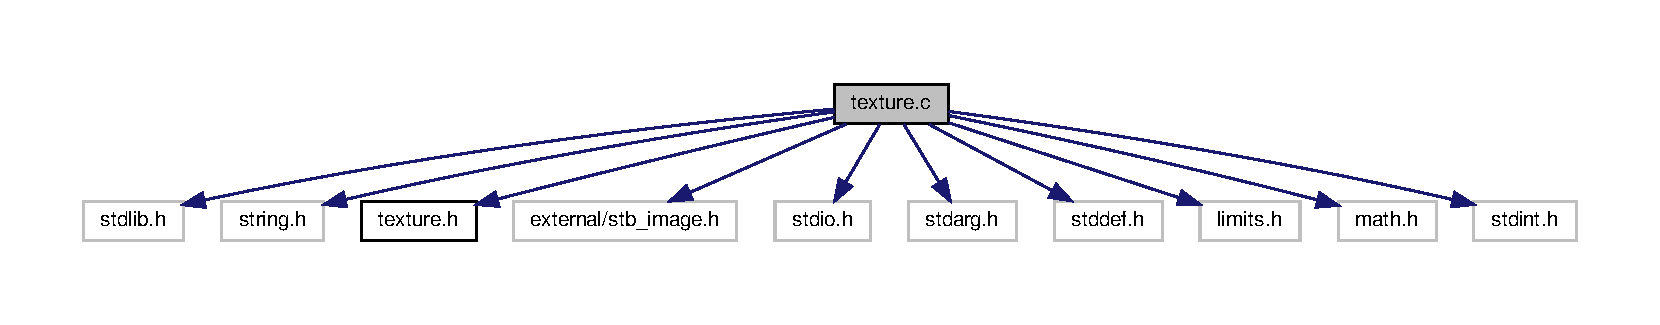
\includegraphics[width=350pt]{texture_8c__incl}
\end{center}
\end{figure}
\subsection*{Macros}
\begin{DoxyCompactItemize}
\item 
\mbox{\Hypertarget{texture_8c_a18372412ad2fc3ce1e3240b3cf0efe78}\label{texture_8c_a18372412ad2fc3ce1e3240b3cf0efe78}} 
\#define {\bfseries S\+T\+B\+\_\+\+I\+M\+A\+G\+E\+\_\+\+I\+M\+P\+L\+E\+M\+E\+N\+T\+A\+T\+I\+ON}
\item 
\mbox{\Hypertarget{texture_8c_abcf0d8bc32a73fd449d918aac2ed3882}\label{texture_8c_abcf0d8bc32a73fd449d918aac2ed3882}} 
\#define {\bfseries S\+T\+B\+I\+\_\+\+A\+S\+S\+E\+RT}(x)
\end{DoxyCompactItemize}
\subsection*{Functions}
\begin{DoxyCompactItemize}
\item 
\mbox{\Hypertarget{texture_8c_abb654b7f7e436f514304c9a0cba313b3}\label{texture_8c_abb654b7f7e436f514304c9a0cba313b3}} 
struct \hyperlink{structtexture}{texture} $\ast$ {\bfseries Texture\+Init\+From\+File} (char $\ast$file)
\item 
\mbox{\Hypertarget{texture_8c_ac4f675bcddb203ea0adf6601c208b49a}\label{texture_8c_ac4f675bcddb203ea0adf6601c208b49a}} 
void {\bfseries Texture\+Deinit} (struct \hyperlink{structtexture}{texture} $\ast$t)
\item 
\mbox{\Hypertarget{texture_8c_a7ec81fb11654f3d0b6e9eb627091a76a}\label{texture_8c_a7ec81fb11654f3d0b6e9eb627091a76a}} 
unsigned int {\bfseries Texture\+Sample} (struct \hyperlink{structtexture}{texture} $\ast$t, float u, float v)
\end{DoxyCompactItemize}

\hypertarget{texture_8h}{}\section{texture.\+h File Reference}
\label{texture_8h}\index{texture.\+h@{texture.\+h}}
This graph shows which files directly or indirectly include this file\+:\nopagebreak
\begin{figure}[H]
\begin{center}
\leavevmode
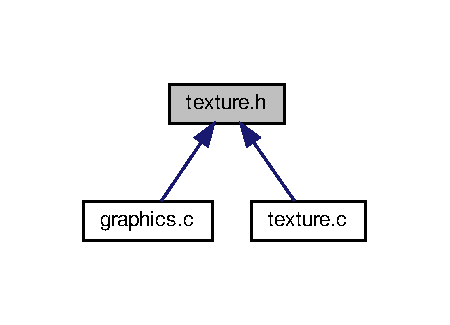
\includegraphics[width=216pt]{texture_8h__dep__incl}
\end{center}
\end{figure}
\subsection*{Classes}
\begin{DoxyCompactItemize}
\item 
struct \hyperlink{structtexture}{texture}
\begin{DoxyCompactList}\small\item\em data is always R\+GB with 8-\/bits per component and no padding in rows. \end{DoxyCompactList}\end{DoxyCompactItemize}
\subsection*{Functions}
\begin{DoxyCompactItemize}
\item 
\mbox{\Hypertarget{texture_8h_abb654b7f7e436f514304c9a0cba313b3}\label{texture_8h_abb654b7f7e436f514304c9a0cba313b3}} 
struct \hyperlink{structtexture}{texture} $\ast$ {\bfseries Texture\+Init\+From\+File} (char $\ast$file)
\item 
\mbox{\Hypertarget{texture_8h_a9d2ab87d8c30cbf53605598654511de1}\label{texture_8h_a9d2ab87d8c30cbf53605598654511de1}} 
void {\bfseries Texture\+Deinit} (struct \hyperlink{structtexture}{texture} $\ast$\hyperlink{structtexture}{texture})
\item 
\mbox{\Hypertarget{texture_8h_a391fe321452fcd146c3287bc5bcee950}\label{texture_8h_a391fe321452fcd146c3287bc5bcee950}} 
unsigned int {\bfseries Texture\+Sample} (struct \hyperlink{structtexture}{texture} $\ast$\hyperlink{structtexture}{texture}, float u, float v)
\end{DoxyCompactItemize}

\hypertarget{triangle__list_8h}{}\section{triangle\+\_\+list.\+h File Reference}
\label{triangle__list_8h}\index{triangle\+\_\+list.\+h@{triangle\+\_\+list.\+h}}
{\ttfamily \#include \char`\"{}math.\+h\char`\"{}}\newline
Include dependency graph for triangle\+\_\+list.\+h\+:\nopagebreak
\begin{figure}[H]
\begin{center}
\leavevmode
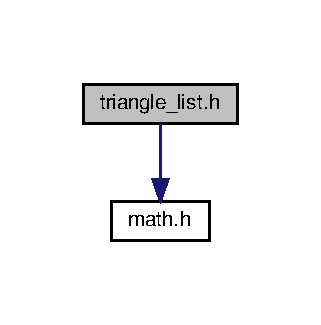
\includegraphics[width=154pt]{triangle__list_8h__incl}
\end{center}
\end{figure}
\subsection*{Classes}
\begin{DoxyCompactItemize}
\item 
struct \hyperlink{structtriangle__list}{triangle\+\_\+list}
\end{DoxyCompactItemize}
\subsection*{Functions}
\begin{DoxyCompactItemize}
\item 
\mbox{\Hypertarget{triangle__list_8h_acad571034d9a457c0c72d7cf78dc31fe}\label{triangle__list_8h_acad571034d9a457c0c72d7cf78dc31fe}} 
struct \hyperlink{structtriangle__list}{triangle\+\_\+list} {\bfseries Triangle\+List\+Init} ()
\item 
\mbox{\Hypertarget{triangle__list_8h_a7e076ba82c1c3aab3245196de4a4f29d}\label{triangle__list_8h_a7e076ba82c1c3aab3245196de4a4f29d}} 
struct \hyperlink{structtriangle}{triangle} {\bfseries Triangle\+List\+Pop\+Front} (struct \hyperlink{structtriangle__list}{triangle\+\_\+list} $\ast$triangle\+List)
\item 
\mbox{\Hypertarget{triangle__list_8h_aaa20c65aa71ff6439ec9dfa293210630}\label{triangle__list_8h_aaa20c65aa71ff6439ec9dfa293210630}} 
void {\bfseries Triangle\+List\+Push\+Back} (struct \hyperlink{structtriangle__list}{triangle\+\_\+list} $\ast$triangle\+List, struct \hyperlink{structtriangle}{triangle} in)
\item 
\mbox{\Hypertarget{triangle__list_8h_af1ed6d69e70a1bc247a1f9649acee02a}\label{triangle__list_8h_af1ed6d69e70a1bc247a1f9649acee02a}} 
int {\bfseries Triangle\+List\+Size} (struct \hyperlink{structtriangle__list}{triangle\+\_\+list} $\ast$triangle\+List)
\end{DoxyCompactItemize}

%--- End generated contents ---

% Index
\backmatter
\newpage
\phantomsection
\clearemptydoublepage
\addcontentsline{toc}{chapter}{Index}
\printindex

\end{document}
